%% Online supplementary material for:
%% Quantum Technologies for Autonomous Robotics: A Systematic Survey of Methods, Evidence, and Deployment Constraints
\documentclass[acmsmall,screen,review]{acmart}
\usepackage{array,booktabs,longtable,xcolor,pdflscape}
\newcommand{\fillin}[1]{{\color{red}[#1]}}
%% Extra stretch lets TeX avoid overfull lines around long words and \texttt names.
\setlength{\emergencystretch}{1.5em}
\setcopyright{none}
\settopmatter{printacmref=false, printccs=false, printfolios=true}
\acmJournal{CSUR}
\renewcommand\thetable{S\arabic{table}}
\renewcommand\thefigure{S\arabic{figure}}
\begin{document}
\title{Online Supplementary Material for ``Quantum Technologies for Autonomous Robotics: A Systematic Survey of Methods, Evidence, and Deployment Constraints''}
\author{Yeshwanth Guru}
\affiliation{\department{Department of Mechanical Engineering}\institution{Amrita Vishwa Vidyapeetham}\city{Chennai}\country{India}}
\author{Dev Kunwar Singh Chauhan}
\affiliation{\department{Department of Mechanical Engineering}\institution{Amrita Vishwa Vidyapeetham}\city{Chennai}\country{India}}
\maketitle
This supplement contains the evidence table for the 72 primary studies (Table~\ref{tab:evidence}), the PRISMA 2020 flow of records (Table~\ref{tab:flow}) and checklist (Table~\ref{tab:prisma}), the quality-assessment rubric (Table~\ref{tab:rubric}) and the per-study appraisal (Table~\ref{tab:appraisal}), and the databases and search strings (Table~\ref{tab:search}). A machine-readable version of the evidence table, which also records where the quantum component of each study was executed, accompanies this supplement. Citations refer to the reference list of the main article.

{\scriptsize
\begin{longtable}{@{}>{\raggedright\arraybackslash}p{0.120\dimexpr\linewidth-12\tabcolsep\relax}>{\raggedright\arraybackslash}p{0.140\dimexpr\linewidth-12\tabcolsep\relax}>{\raggedright\arraybackslash}p{0.180\dimexpr\linewidth-12\tabcolsep\relax}>{\raggedright\arraybackslash}p{0.170\dimexpr\linewidth-12\tabcolsep\relax}>{\raggedright\arraybackslash}p{0.210\dimexpr\linewidth-12\tabcolsep\relax}>{\raggedright\arraybackslash}p{0.180\dimexpr\linewidth-12\tabcolsep\relax}@{}}
\caption{Evidence table for the 72 primary studies. The evidence level (Table 2 of the main article) is given in parentheses after each study; ``sim.'' denotes a simulated robot environment; $^\dagger$ marks studies available only as preprints when they were graded.}\label{tab:evidence}\\
\toprule
\textbf{Study (level)} & \textbf{Robotic task; quantum type} & \textbf{Method} & \textbf{Setup and data} & \textbf{Key result} & \textbf{Limitation} \\ \midrule
\endfirsthead
\toprule
\textbf{Study (level)} & \textbf{Robotic task; quantum type} & \textbf{Method} & \textbf{Setup and data} & \textbf{Key result} & \textbf{Limitation} \\ \midrule
\endhead
\bottomrule
\endfoot
\citet{Petschnigg2019} (Review) & Robotics in general; \emph{Position paper / survey} & Survey of where quantum algorithms could affect robotics & --- & Maps quantum ML, quantum image processing, optimization (trajectory planning, task allocation, kinematics), sensing/perception and system diagnosis to robot functions; lists open problems & Speculative; most cited speed-ups (e.g., quantum PCA, quantum image processing) assume fault-tolerant hardware and qRAM \\
\citet{Tandon2017} (Review) & Robotics in general; \emph{Book / survey} & Monograph surveying quantum mechanisms relevant to robot sensing, planning, learning and acting & --- & Covers quantum search, quantum Markov decision processes, quantum RL, quantum sensing and control, and quantum-scale manipulation; offers a roadmap & Predates most NISQ-era experimental work (2019 onwards) \\
\citet{Yan2024} (Review) & Robotics in general; \emph{Review} & Review of quantum robotics: architectures, perception and robot--environment interaction & --- & Covers quantum path planning, quantum-inspired inverse kinematics, quantum RL navigation, QML, quantum sensors, multi-robot coordination, quantum affective computing, quantum image processing and quantum-secure communication & Broad and largely descriptive; limited critical assessment of hardware feasibility \\
\citet{Nigatu2026} (Review) & Robotics in general (QML focus); \emph{Review} & Review of 107 contributions on QML for robotics & --- & Organises the field into QRL for navigation/control, quantum search and path planning, quantum-enhanced localization and mapping, quantum optimization for IK and task allocation, and multi-robot coordination & QML-centerd; limited treatment of sensing, cognition and deployment latency \\
\citet{Udekwe2025}$^\dagger$ (Review) & Robotics in general; \emph{Review} & Systematic review guided by four research questions; robotics tasks recast as optimization, search, sampling and linear-algebra problems & --- & Covers annealing and variational control, Grover-type search and quantum-inspired sampling, QML for perception and RL, and hardware/latency constraints & Preprint \\
\citet{Fazilat2025a} (Review) & Robot control; \emph{Review} & Brief survey of quantum-oriented control: QNNs, QML, QPSO, quantum RL, distributed NISQ and hybrid approaches & --- & Maps quantum-assisted adaptive control, trajectory planning and optimization methods & Short conference review; much of the covered work is quantum-inspired \\
\citet{Haldorai2024} (Review) & Robotics in general; \emph{Review} & Narrative review of quantum computing principles and applications in robotics, AI, data mining and image processing & --- & Highlights integration needs and scale-up challenges & Descriptive; lower-impact venue \\
\citet{Benioff1998} (L1) & Quantum robot concept: a mobile quantum system with an onboard quantum computer that interacts with its environment; \emph{Quantum (theoretical model)} & Formal model of quantum robots and the environments they act in & --- & Introduces the quantum robot and describes how it can carry out tasks through interactions with its environment & Theoretical; robot and environment are both quantum systems, with no link to classical robot hardware \\
\citet{Benioff2002} (L1) & Search of a two-dimensional region by a quantum robot; \emph{Quantum (theoretical model)} & Analysis of Grover-type search carried out by a quantum robot that must move through the region it searches & --- & A quantum robot's Grover search of a two-dimensional region is no faster than a classical search, because the robot's motion cancels the query advantage & Theoretical; assumes an idealized quantum robot \\
\citet{Dong2006} (L2) & Robot learning and control; \emph{Conceptual architecture + simulation} & Quantum robot architecture with multi-quantum computing units (MQCU), quantum controller/actuator and information acquisition units; Grover-based search and quantum reinforcement learning & Theoretical complexity analysis and simple learning simulations & Grover search lowers search complexity quadratically; simulated quantum RL learned more efficiently than a classical learner & Assumes idealised on-board quantum hardware; small illustrative simulations \\
\citet{Ohzeki2019} (L3) & Multi-AGV collision-free routing in a factory; \emph{Quantum annealing (D-Wave 2000Q) + digital annealer} & Route selection for all AGVs posed as a QUBO with penalty terms for one-route-per-AGV and no simultaneous occupation of intersections; re-solved every time period & Simulation of a real DENSO plant layout with 10 AGVs ($\leq$60 binary variables); D-Wave 2000Q, Fujitsu Digital Annealer and Gurobi compared with the conventional rule-based control & QUBO control gave smoother, collision-free traffic than the conventional rule; D-Wave produced plans in a short time but only for few vehicles; digital solvers handled larger instances quickly & Small problem size on quantum hardware; post-processing needed to repair infeasible annealer outputs; classical solvers remained competitive or better \\
\citet{Quang2025} (L4 (sim.)) & Large-scale AGV fleet routing (warehouse); \emph{Quantum annealing (D-Wave, cloud) + classical and quantum-inspired solvers} & Real-time candidate-route generation, priority-weighted QUBO, and dynamic problem clustering that splits the fleet into sub-QUBOs; integrated with a commercial AGV operating system & Commercial AGV operating-system layout (154 m $\times$ 298 m, 8,242 tags) with real warehouse request data; AGV simulator with up to 1,000 AGVs & Route generation cut variables by 96\% (small/medium) and 78\% (large systems); clustering capped subproblems below 10,000 variables; complexity-based formulation reduced sampling time ~28\% & Fleet behavior simulated; no head-to-head speed comparison showing a quantum advantage over classical solvers \\
\citet{Clark2019} (L3) & Multi-robot routing on a grid; \emph{Quantum annealing (D-Wave 2000Q) hybrid} & Hybrid pipeline: classical computation generates candidate paths per robot; quantum annealing (QUBO) selects the conflict-free combination of paths & Grid-world routing benchmarked classically and on a D-Wave 2000Q with up to 200 robots & Valid (collision-free) multi-robot routing solutions obtained with current quantum annealing hardware for up to 200 robots & Discrete grid; embedding and connectivity limits of the annealer; real-time claim not supported by end-to-end latency including cloud access \\
\citet{Smierzchalski2024} (L3) & AGV scheduling in a factory; \emph{Quantum annealing hybrid (D-Wave CQM)} & AGV scheduling mapped to a railway-style scheduling model and solved with D-Wave hybrid (CQM) solvers & Realistic factory scenario, up to 21 AGVs and 7 zones (~1,300 variables); CPLEX baseline & Hybrid solver handled 21 AGVs in seconds and was comparable to classical solvers; AGV problems are sparser and better suited to QC than railway problems & Proprietary hybrid solver, so the contribution of the QPU itself is unclear; CPLEX competitive \\
\citet{Leib2023} (L3) & Transport-robot scheduling in a laboratory; \emph{Quantum annealing hybrid (D-Wave) vs quantum-inspired (Fujitsu DA) vs classical (Gurobi)} & Three QUBO/MIP models of a transport-robot scheduling problem from a BASF high-throughput laboratory, benchmarked across solvers on end-to-end runtime and solution quality & Large instance set of varying difficulty; D-Wave hybrid, Fujitsu Digital Annealer (and hybrid), Gurobi & Gurobi reached comparable quality 10--100$\times$ faster on smaller instances; Fujitsu's quantum-inspired hybrid was better on the largest instances; D-Wave showed only some opportunities & Advantage, where found, came from quantum-inspired digital hardware rather than a quantum device \\
\citet{AtchadeAdelomou2021} (L3) & Warehouse order picking and batching for mobile robots; \emph{Quantum (VQE/QAOA and annealing via cloud; simulators)} & Picking/batching modeled as a capacitated vehicle-routing QUBO (docplex) and solved with VQE and other hybrid algorithms; robot controller on a Raspberry Pi 4 calling cloud QPUs & Proof of concept with small warehouse instances; IBM Q, Amazon Braket, D-Wave and PennyLane back-ends & Demonstrated an end-to-end robot-to-cloud quantum pipeline that returns valid routes for small instances & Very small instances; no systematic comparison with classical VRP solvers; cloud latency not addressed for real-time use \\
\citet{Windmann2023} (L3) & Job scheduling for automated storage and retrieval systems; \emph{Quantum (QAOA on IBM Q System One)} & Scheduling formulated as an asymmetric QUBO and solved with QAOA & IBM Q System One (Ehningen); running time and qubit scalability study & Running time and qubit requirements quantified for small scheduling instances & Small instances; scalability limited by qubit count \\
\citet{Schuetz2022} (L3) & Industrial robot trajectory (sequencing) planning in automotive manufacturing; \emph{Quantum annealing (Amazon Braket, qbsolv) within a classical pipeline} & Biased random-key genetic algorithm with model stacking, ensembles and path relinking; quantum annealing complement via qbsolv on Amazon Braket & Industry-scale BMW data sets & Classical pipeline consistently outperformed greedy baselines; annealing results integrated as a quantum-ready module & Nearly all of the performance comes from the classical algorithm; quantum hardware used only on reduced sub-problems \\
\citet{Willmann2025} (L3) & Robotic assembly line balancing; \emph{Quantum annealing (D-Wave Advantage 4.1)} & Integer program reformulated as a QUBO and solved with a hybrid annealing workflow (QBSolv) & Small case: 4 tasks, 2 workstations, 2 equipment types & Optimal solutions found among samples, but total quantum workflow took ~10,110 s versus 0.03 s for the exact classical solver & Toy instance; communication overhead dominates; connectivity and noise limit scale \\
\citet{Osaba2025} (L3) & Robotic quality-inspection path planning from CAD models; \emph{Quantum annealing hybrid (D-Wave CQM and NL solvers)} & Inspection trajectory modeled as a 3D open-route TSP on incomplete graphs; D-Wave hybrid solvers compared with Gurobi and Google OR-Tools & Five real industrial inspection cases & Competitive solution quality with significantly reduced computation time reported for the hybrid NL solver & Short paper; hybrid solvers are proprietary; limited detail on runtimes \\
\citet{Otani2025} (L3) & Manipulator inverse kinematics / posture optimization; \emph{Quantum (gate-based; simulator + 64-qubit superconducting hardware)} & Forward kinematics of each link encoded in a qubit via rotation gates, parent--child link coupling via entangling (RXX/RYY/RZZ) gates; joint angles optimized with classical COBYLA & Two-link manipulator with 3 rotational DOF per joint; Qiskit simulation and the RIKEN/Fujitsu 64-qubit superconducting computer & Adding entanglement reduced end-effector position error and sped up convergence, both in simulation and on hardware & Only rotational joints; one-directional parent-to-child dependency; very small (2-qubit) problem; no comparison of accuracy or speed with classical IK solvers \\
\citet{Salloum2026} (L3) & Manipulator inverse kinematics; \emph{Quantum annealing (D-Wave Pegasus/Zephyr) + hybrid} & Planar IK reformulated as QUBO via linear binary discretization of joint angles with one-hot constraints; embedding strategies compared & Two-link planar IK instances on D-Wave Pegasus and Zephyr; classical QUBO baselines; rigorous time-to-solution & Global embedding on Zephyr used fewest qubits and shortest access time; hybrid solver had lower time-to-solution than classical QUBO baselines at larger sizes & Authors explicitly do not claim superiority over continuous IK solvers; planar two-link case only \\
\citet{Wang2025} (L2 + real data) & Regression testing of autonomous mobile robot software; \emph{Quantum (quantum reservoir computing, simulated) with industrial robot data} & QuReBot: quantum reservoir computing combined with a lightweight classical network to predict expected robot behavior as a test oracle & Industrial AMR data from PAL Robotics; classical neural-network baseline & QRC alone failed to converge; QuReBot converged and reduced prediction error (MSE) by ~15\% versus the classical baseline & Simulated quantum reservoir; single industrial robot and task \\
\citet{Roh2025} (L2 + real data) & Object detection for autonomous driving; \emph{Quantum (simulated QCNN) with real driving data} & Fast quantum convolution that uploads input-channel information to cut qubit and circuit cost; quantum convolution-based object detection (QCOD) & KITTI autonomous-driving dataset; simulated quantum circuits & Object detection on KITTI with reduced computational complexity & Simulated circuits; no on-vehicle or QPU deployment \\
\citet{Goncalves2018}$^\dagger$ (L3) & Quantum robot interacting with a quantum target; \emph{Quantum (IBM 5-qubit hardware) + theory} & Quantum neural networks under a 'quantum force' interpretation; quantum optimization of a conditional utility function for a quantum robot's adaptive control & Examples on IBM's five-qubit transmon chip via IBM Q Experience & Demonstrates implementability of small quantum neural networks and a quantum-robot control scheme on real hardware & Highly theoretical; tiny circuits; no classical comparison \\
\citet{Dong2012} (L5) & Mobile-robot navigation; \emph{Quantum-inspired (classical hardware)} & Quantum-inspired RL (QiRL): action selection by 'collapse' of an action superposition; amplitude-amplification-style reinforcement of good actions & 58-state Markov grid; 600$\times$400-grid simulated navigation; real two-wheeled MT-R robot & Converged in ~2,000 episodes; more robust to learning rate and initial state than TD learning; learned obstacle avoidance faster than TD in simulation and on a real robot & Runs entirely on a classical computer; compared only with basic TD learning; small discrete state spaces \\
\citet{Hohenfeld2024} (L4 (sim.)) & Mobile-robot navigation; \emph{Quantum (simulated PQC)} & Hybrid quantum DDQN: parameterized quantum circuit (PQC) as Q-function approximator; two data-encoding schemes compared & Simulated Turtlebot 2 in three static grid environments and a large dynamic lidar environment; classical DDQN neural-network baseline & PQCs learned optimal policies with far fewer trainable parameters and beat parameter-matched classical networks; the larger classical network was faster, more stable and better in the dynamic environment & Idealised noise-free simulation; no quantum hardware; advantage only when parameter counts are equalised \\
\citet{Dragan2025} (L4 (sim.)) & Mobile-robot maze navigation (continuous control); \emph{Quantum (simulated VQC)} & DDPG with variational quantum circuits (horizontally shifting data re-uploading) as actor and critic; continuous wheel-velocity actions from LiDAR inputs & Simulated Turtlebot 2 in 3$\times$3, 4$\times$4 and 5$\times$5 warehouse-like mazes; 4 and 8 qubits; classical DDPG (256$\times$256) baseline & Best quantum model (8 qubits, 851 parameters) solved 3$\times$3 and 4$\times$4 mazes 30/30 but 5$\times$5 only 10/30; classical DDPG (136,451 parameters) solved all 30/30; ~200$\times$ fewer parameters & Classical baseline better on the hardest maze and in step efficiency; simulation only; more qubits/layers did not consistently help \\
\citet{Sinha2023} (L4 (sim.)) & Autonomous-driving collision-free navigation; \emph{Quantum (simulated PQC, incl. noisy simulation)} & Nav-Q: actor--critic DRL in which the critic is a hybrid quantum--classical network; new QIDEP data-encoding extending data re-uploading & CARLA-CTS1.0 driving benchmark; classical NavA2C baseline; ideal and noisy quantum simulation & More stable training across initializations and sometimes faster convergence than NavA2C with far fewer parameters; higher effective dimension; noise degraded training but increased exploration & Simulation only; quantum part used only in training (critic), so any benefit is to training, not to on-board inference \\
\citet{Acuto2022}$^\dagger$ (L4 (sim.)) & Robotic-arm continuous control; \emph{Quantum (simulated VQC)} & Variational quantum Soft Actor-Critic (QSAC): actor and/or critics replaced by variational quantum circuits & Simulated robotic arm reaching task; classical SAC baselines with matched and 100$\times$ parameter counts & Fully quantum QSAC (~2,700 parameters) converged, whereas a classical SAC with ~3,000 parameters did not; classical SAC needed ~100$\times$ more parameters (~274k) to match & Digital simulation only; single simple arm task; with a quantum actor alone there was no learning advantage; preprint \\
\citet{Lokossou2025}$^\dagger$ (L4 (sim.)) & Legged/\allowbreak humanoid locomotion-navigation (MuJoCo Walker2d); \emph{Quantum (simulated PQC)} & Variational quantum soft actor-critic with parameterized quantum circuits & MuJoCo Walker2d-v4; classical SAC baseline; 17-qubit circuits in simulation & Quantum SAC reached ~8\% higher average return than classical SAC with far fewer training steps, using 41 vs 1,250 learnable parameters & Simulation only; Walker2d rather than full humanoid because of qubit limits; single environment \\
\citet{Altrabulsi2026}$^\dagger$ (L3) & Mobile-robot navigation with dynamic obstacles; \emph{Quantum (simulated + IBM hardware execution)} & Q-SpiRL: quantum-enhanced spiking neural network (QSNN) combining spike-based temporal processing with an 8-qubit variational circuit & 20$\times$20, 30$\times$30 and 40$\times$40 grid worlds with static/dynamic obstacles; tabular Q-learning, MLP, SNN and quantum-MLP baselines & QSNN gave the best trade-off of success, path efficiency and smoothness, up to 99\% success in the hardest setting; policy executed on IBM quantum hardware & Discrete grid worlds; hardware run is a feasibility demonstration, not training on hardware; preprint \\
\citet{Taghavi2025} (L4 (sim.)) & Multi-UAV navigation (safe MARL); \emph{Quantum (simulated VQC) + neuromorphic SNN} & CTDE multi-agent RL: variational quantum circuits for high-level policy exploration and spiking neural networks for low-latency control & Simulated forest environment with ten UAV agents, limited visibility and obstacles; classical MARL baselines & Fewer safety violations while maintaining exploration and interpretability, relative to classical MARL baselines & Simulation only; lower-impact venue; quantum contribution not isolated from the SNN component \\
\citet{Park2023} (L4 (sim.)) & Cooperative mobile access with multi-UAV fleets; \emph{Quantum (simulated VQC) multi-agent RL} & Quantum multi-agent actor-critic networks with a quantum centralized critic & Simulated multi-UAV mobile-access environment; classical MARL baselines & Faster training and better wireless service quality than classical baselines with fewer parameters & Simulated circuits and environment; communication-centric task \\
\citet{Park2024} (L4 (sim.)) & Cooperative autonomous mobility (multi-agent); \emph{Quantum (simulated VQC) multi-agent RL} & Quantum MARL actor-critic with projection-value-measure action reduction & Simulated multi-agent mobility scenario & Parameter-efficient training and fast convergence; the projection-value measure reached the highest reward by reducing the action dimension to logarithmic scale & Magazine-length evaluation; simulation only \\
\citet{Sun2025}$^\dagger$ (L5) & Real-time balance control of a physical cart-pole; \emph{Quantum (simulated VQC) on physical control hardware} & Model-based offline policy search with a pure VQC policy (trainable input and output weights) in place of an MLP & Hardware cart-pole driven by a Raspberry Pi and an Arduino; VQC executed by local classical simulation; latency compared with IBM cloud execution & Quantum policies balanced the hardware cart-pole; local simulated execution met the real-time deadline, whereas cloud QPU execution took seconds & Circuit simulated classically; single toy system; cloud QPU too slow for closed-loop control \\
\citet{Ngo2026}$^\dagger$ (L3) & Cart-pole balancing (control benchmark); \emph{Quantum (single-qubit VQC on the VTT Q5 superconducting QPU)} & Actor-critic policy gradient with a five-gate single-qubit variational circuit; readout electronics programmed directly through command tables & CartPole benchmark; VTT Q5 five-qubit processor with Zurich Instruments control electronics & Bypassing the standard software stack made circuit execution more than ten times faster; the single-qubit agent learned in fewer episodes than the classical baseline & Throughput still below the tens of hertz needed for closed-loop control; one-qubit agent on a benchmark task \\
\citet{Chella2022} (L2) & Single-robot motion/path planning; \emph{Quantum (gate-based, simulated)} & Robot behavior encoded as a production system; plans found by Grover search over the action tree using a reversible Boolean oracle; qubit-reuse technique for simulation & Grid map with fixed obstacles; Qiskit Aer noiseless simulator on a 16 GB laptop ($\approx$27-qubit limit) & Correct plans found with high success probability; quadratic reduction in search queries $O(\sqrt{N})$ versus exhaustive tree search & Noise-free simulation only; qubits grow with plan depth; oracle construction assumes a known map; no comparison with classical planners such as A* or RRT \\
\citet{Chella2023} (L2) & Swarm path planning (search and rescue); \emph{Quantum (gate-based, simulated)} & Quantised position/reward information; pairwise information exchange as a quantum logic gate; per-robot Grover-based path planning (extends Chella et al., 2022) & Ant-foraging search-and-rescue scenario; Qiskit simulation; compared with NetLogo and Java ant-colony simulations & Faster convergence of the swarm to the target than both classical ant-behavior simulations & Simulation only; small swarms; classical baselines are generic ant simulations rather than optimized swarm planners \\
\citet{Lathrop2023} (L2) & Sampling-based motion planning; \emph{Quantum (Grover-type search; simulated)} & Sampling-based planners recast as database-oracle structures solved by quantum search, including quantum full path search (q-FPS) and quantum RRT (q-RRT) & Simulated planning problems (2D random lattices); q-RRT compared with classical RRT in classical simulation & Quadratic speed-up of q-RRT over RRT confirmed in simulation & Speed-up shown only in classical simulation of the quantum algorithm; a real advantage needs fault-tolerant hardware \\
\citet{Nigatu2025} (L2) & Manipulator kinematic optimization; \emph{Quantum (PQC + Grover; simulated)} & Parameterized circuit trained to approximate forward kinematics, then used as a Grover oracle to search for optimal configurations & Simulated 1-DoF, 2-DoF and dual-arm manipulator tasks; Nelder-Mead and other classical optimizers as baselines & Quadratic reduction in search complexity; up to 93$\times$ speed-up over Nelder-Mead as dimensionality grew (simulated) & Simulation only; speed-up counted in model evaluations/oracle queries rather than wall-clock time on hardware \\
\citet{Sarkar2024} (L2) & Mobile-robot multi-target path planning (TSP); \emph{Hybrid quantum ant-colony optimization (Qiskit simulation / Amazon Braket)} & Hybrid Quantum Ant Colony Optimization (HQACO): quantum circuits generate ant tours automatically from classical data, running ants in parallel on a hybrid architecture & TSPLIB instances and 50 random 16-node graphs; Qiskit simulator, Amazon Braket for larger circuits; OR-Tools optimum as reference & Optimal or near-optimal tours, with average error of about 7\% from the optimum & Simulated circuits; error grows with qubit count; no runtime advantage shown \\
\citet{Gerlach2025} (L3) & Optimal multi-agent pathfinding (MAPF); \emph{Quantum (QUBO subproblems; real quantum hardware + classical)} & Branch-and-cut-and-price MAPF in which conflict-resolution subproblems are solved as QUBOs over conflict graphs (QUBO-and-Price, QUBO-Cut-and-Price) & Standard MAPF benchmarks; experiments on real quantum hardware; compared with BCP, EECBS, LaCAM* and LNS2 & First optimal hybrid quantum--classical MAPF algorithms; outperformed earlier QUBO formulations and, on the reported benchmarks, state-of-the-art MAPF solvers & Advantage depends on problem structure and small QUBO sizes; hardware results limited to small instances \\
\citet{Innan2025}$^\dagger$ (L3) & UAV path planning with obstacle and no-fly-zone avoidance; \emph{Quantum (QAOA; simulation + IBM ibm\_kyiv)} & Pathfinding encoded as QAOA cost Hamiltonian with obstacle constraints and geospatial coordinate transformation & Simulations and a real-hardware run on IBM ibm\_kyiv & Feasible, efficient trajectories generated despite hardware noise; circuit depth scales linearly with the number of graph edges & Small graphs; no comparison of quality or runtime against classical planners such as A* \\
\citet{OsabaDrone2025} (L3) & Drone routing with real-world constraints; \emph{Quantum (QAOA via Eclipse Qrisp and D-Wave annealers)} & Two-phase Q4DR: QAOA-based clustering followed by annealer-based routing & Three use cases of increasing complexity with asymmetric costs, forbidden paths and charging points & Feasible routes for all three use cases & Small use cases; quantum contribution not isolated from the classical decomposition \\
\citet{Bang2026}$^\dagger$ (L2) & Multi-drone task assignment from natural-language instructions; \emph{Quantum (CVaR-QAOA; statevector simulation)} & Fine-tuned LLM maps instructions to QUBO constraints; W-state initialization and XY mixers preserve assignment constraints; constraint-preserving partitioning with a separator-based dynamic-programming merge & Statevector simulation of decomposed sub-QUBOs & Global optimum in 100\% of oracle evaluations and 96.3\% of cases with CVaR-QAOA sampling & Simulation only; hardware runs left to future work \\
\citet{Rao2024}$^\dagger$ (L2) & Multi-vehicle coverage path planning; \emph{Quantum (gate-based QAOA design; resource estimates)} & Objective function and constraint-preserving Quantum Alternating Operator Ansatz operators for exploring grid paths; validity proofs and resource estimation & 2D grid instances; comparison with depth-first search & Reported runtime improvements over DFS-based exploration; resource estimates for current hardware & Theoretical/\allowbreak simulated; comparison against DFS rather than state-of-the-art coverage planners \\
\citet{GonzalezVillasmil2026}$^\dagger$ (L2) & Multi-robot path planning; \emph{QUBO (simulated annealing; simulated QAOA)} & Joint QUBO for multiple robots with BFS-based variable pruning (>95\% reduction) and time-windowed decomposition & Grids up to 10$\times$10 with up to four robots; D-Wave simulated annealing and PennyLane-simulated QAOA & Near-optimal paths (5.3\% length penalty in dense scenarios); classical planners remained faster at tested sizes & No quantum hardware; small grids; single-author preprint \\
\citet{Yu2025} (L2) & Robotic view planning / next-best-view exploration; \emph{Quantum (variational, simulated)} & Multi-term Hamiltonian for viewpoint selection with a parameter-centric variational ansatz using bidirectional alternating entanglement & Simulated exploration of diverse environments with obstacles; classical view-planning baselines & 7.9--49.2\% higher exploration efficiency than classical methods; ablations attribute gains to entanglement structure & Simulated quantum circuits; preprint; baselines not state-of-the-art NBV planners \\
\citet{Antero2025} (L3) & Mobile-robot localization; \emph{Quantum (gate-based; simulator + real devices)} & Localization cast as pattern search: the robot's local perception costmap is matched against a pre-built map costmap with a Grover-search oracle & Small 2D grid maps; Qiskit simulation ($\leq$40 qubits) and cloud quantum devices; compared with Monte Carlo localization (MCL) & Correct localization in simulation; theoretical $O(\sqrt{N})$ vs O(N) query scaling over map cells; accuracy on real devices degraded as map size grew & Claimed speed-up is asymptotic query count, not measured wall-clock time; simulation capped at ~40 qubits; real-device noise limits map size; preprint \\
\citet{Cheiney2018} (L3 (lab)) & Inertial navigation (accelerometer bias tracking); \emph{Quantum sensing (laboratory hardware)} & Hybrid sensor: cold-atom matter-wave interferometer continuously corrects the bias drift of a classical accelerometer via a Kalman filter & Laboratory set-up with experimentally simulated harsh, mobile-like vibration environment & More precise and robust than sine-fitting; 400 Hz bandwidth with 10 ng stability after 11 h of integration & Laboratory demonstration; single axis; size and power of cold-atom hardware remain barriers for mobile robots \\
\citet{Templier2022} (L3 (lab)) & Inertial navigation (three-axis acceleration); \emph{Quantum sensing (laboratory hardware)} & Three orthogonal atom interferometers hybridized with a navigation-grade classical accelerometer triad & Laboratory demonstration & Acceleration vector at 1 kHz with magnitude accuracy below 10 $\mu$g and 4 $\mu$rad pointing accuracy; 50-fold stability gain over classical accelerometers & Laboratory set-up; not yet on a moving platform \\
\citet{Wang2021}$^\dagger$ (L2) & Inertial navigation (sensor fusion); \emph{Quantum sensing (simulation)} & Maximum-likelihood probabilistic fusion that unwraps the phase of a cold-atom accelerometer using a co-located classical accelerometer, then recalibrates the classical sensor & Simulated 1D inertial navigation scenario & Extended the usable dynamic range of the quantum accelerometer and reduced navigation error compared with classical-only sensing & 1D simulation only; fusion errors when phase ambiguity is large \\
\citet{Wang2023} (L2) & GNSS-denied navigation (magnetic map matching); \emph{Quantum sensing (simulation)} & Diamond (NV-center) magnetometer measurements with probabilistic data association and multiple-hypothesis/Viterbi map-matching filters to aid an IMU & Simulations at current and near-term diamond magnetometer sensitivities; scalar and vector magnetometry & Quantifies expected navigation errors and shows vector diamond magnetometry can bound INS drift & Simulation only; depends on magnetic anomaly map quality \\
\citet{Muradoglu2025}$^\dagger$ (L6) & GNSS-denied navigation (aircraft, drones, ground vehicles); \emph{Quantum sensing (field-deployed hardware)} & Magnetic-anomaly navigation using proprietary quantum magnetometers plus denoising and map-matching algorithms that learn platform parameters online & Flight trials from ground level to ~19,000 ft with onboard/outboard sensors; ground-vehicle trial with public anomaly maps; strategic-grade INS as comparator & Up to ~46$\times$ lower positioning error than a velocity-aided strategic-grade INS (best final error 22 m, 0.006\% of distance); $\geq$11$\times$ better across airborne trials; ~7$\times$ better in the ground vehicle & Company-led preprint (Q-CTRL); depends on quality of magnetic-anomaly maps; periodic fixes rather than continuous high-rate positioning \\
\citet{Khoshnoud2020}$^\dagger$ (L5 (lab)) & Cooperative multi-robot autonomy (aerial and ground); \emph{Quantum communication hardware on robots (laboratory)} & Photon-based quantum capabilities (SPDC single photons, polarisation, single-photon detection, entanglement and cryptography concepts) integrated into networks of classical aerial and ground robots & Laboratory demonstrations on classical aerial and ground robotic platforms & Shows the feasibility of carrying quantum-optical communication hardware on cooperating robots & Conceptual/\allowbreak laboratory scale; no quantitative performance comparison \\
\citet{Tian2023} (L5) & Secure communication for aerial robots; \emph{Quantum communication (field experiment on a drone)} & Compact polarisation-encoded decoy-state BB84 QKD transmitter on an octocopter & Drone ($\leq$30 kg take-off weight) to ground over 200 m & Real-time QKD with an average secret-key rate of 8.48 kHz & Short range; single drone; focus on communication rather than autonomy \\
\citet{Liu2021} (L5) & Mobile entanglement distribution between drones; \emph{Quantum communication (field experiment on drones)} & Entangled-photon source on one drone and an optical relay on a second drone & Drone-to-drone relayed link over 1 km & Entanglement distribution at 1 km with CHSH $S=2.59\pm0.11$, above the classical bound & Short range; no robotic task built on the link \\
\citet{Conrad2025}$^\dagger$ (L5) & Secure communication between drones and ground vehicles; \emph{Quantum communication (field deployment on moving platforms)} & Modular, platform-agnostic, reduced-SWaP QKD transmitter and receiver with device models for mobile non-idealities & Drone-to-drone, drone-to-vehicle and vehicle-to-vehicle links & Finite-key secure key rates of 1.6--20 kbps between moving platforms & Communication only; ranges and conditions limited \\
\citet{Widdows2023} (L3) & Cognitive decision-making (order effects, uncertainty); \emph{Quantum cognition model on quantum hardware} & Quantum-probability cognitive models (question-order effects, decisions under uncertainty) implemented as small qubit circuits with gates and measurements & Circuits run on an 11-qubit IonQ trapped-ion computer and simulators & Very small circuits (some a single qubit) reproduce human order effects and non-classical decision patterns & Models are small enough to simulate classically, so no computational advantage is claimed; not applied to robots \\
\citet{Yan2021} (L2) & Robot emotion modeling / multi-robot emotion fusion; \emph{Quantum-formalism model (simulated)} & Emotions encoded as qubit superposition states in an emotion space; unitary operators model emotion transitions; entanglement fuses the emotions of multiple robots & Mathematical framework with small simulation-based demonstrations & Entanglement-based fusion reduces the qubits and gates needed to represent and update the joint emotional state of a robot group & Conceptual; no psychological validation, no physical robots, no comparison with classical affective models \\
\citet{DeCarolis2025} (L1) & Social robotics / human--robot interaction; \emph{Review / position (no experiments)} & Literature review (>35 articles, 2021--2025) and project proposal for quantum-enhanced HRI & --- & Identifies emotion recognition, path finding and cognitive modeling as candidate uses of Grover search and quantum walks in social robots & Short position paper; no implementation or evaluation yet \\
\citet{Daglarli2025} (L2) & Autonomous agent behavior (embodied simulation); \emph{Quantum algorithms in a cognitive architecture (simulated)} & Prefrontal-cortex-inspired cognitive architecture with transformer-based RL and quantum routines (Deutsch--Jozsa, Bernstein--Vazirani, Grover) for decision-making, meta-cognition and situation awareness & Minecraft-based simulation environment with multi-objective exploration tasks & About 2$\times$ faster convergence to 80\% task success and ~15\% higher cumulative reward than the classical agent & Simulated circuits; game environment; the role of each quantum routine is not isolated \\
\citet{Lawless2023} (L1) & Autonomous human--machine (robot) teams; \emph{Quantum-like cognition model (theoretical review)} & Quantum-like interdependence theory: team states are non-separable (entangled-like), and measuring individuals cannot reconstruct team performance & --- & Argues that interdependence, not individual aggregation, explains team performance under complexity, uncertainty and conflict & Theoretical; no quantitative robot experiments \\
\citet{Humr2025} (L1) & Human-in-the-loop AI decision support; \emph{Quantum-probability decision model (perspective)} & Quantum probability theory applied to human rationalisation of AI outputs (order and interference effects, ontic uncertainty) & Illustrative case study & Shows how QPT predicts oscillating, order-dependent beliefs that classical models miss & Perspective paper; not robot-specific; no empirical test \\
\citet{Essalmi2026}$^\dagger$ (L2) & Interaction-aware decision-making for automated driving; \emph{Quantum game model (classically simulated)} & Multi-player, multi-strategy quantum game combining classical game theory with superposed and entangled strategies & Simulated interactive driving scenarios; classical game-theoretic baselines & Higher success rates and fewer collisions than classical approaches, especially in highly interactive scenarios & Simulation only; no human-in-the-loop or vehicle tests \\
\citet{Zuo2018} (L2 + real dataset) & SLAM; \emph{Quantum-inspired (classical hardware)} & QPSO-FastSLAM: quantum-behaved particle swarm optimization (with Gaussian disturbance) refines the particle proposal distribution; diversity-triggered linear-optimization resampling & Bailey's FastSLAM simulator (90 m $\times$ 70 m, 18 landmarks, 20 Monte Carlo runs); Victoria Park outdoor data set & Lower pose and landmark RMSE than FastSLAM 2.0 and PSO-FastSLAM (e.g., 0.44 m vs 0.52 m with 20 particles); same accuracy with fewer particles & Runs on classical hardware (quantum-inspired only); compared only with FastSLAM variants \\
\citet{Fazilat2025b} (L2) & Inverse kinematics of a 6-DoF industrial arm; \emph{Quantum-inspired (classical hardware)} & Multi-layer perceptrons with a quantum-inspired activation function, compared with classical ANNs & ABB IRB140 model (DH parameters) in RobotStudio; singularity-free and singularity-avoidance data sets & 15.6--16.7\% lower mean absolute error than classical ANNs; 1.64 mm position and 0.00179 rad orientation accuracy & Despite the name, no quantum hardware or circuit; runs entirely classically \\
\citet{Mannone2022} (L3) & Swarm modeling; \emph{Quantum (gate-based; IBM simulators and QPUs)} & Category-theoretic classification of swarms and a block-matrix model whose off-diagonal (pairwise) terms are computed with a 4-qubit circuit & Toy model run in IBM Quantum Composer on simulators and real IBM quantum computers & Worked example linking local pairwise quantum interactions to global swarm behavior & Toy model; no performance comparison \\
\citet{Mannone2023} (L3) & Swarm modeling (ant foraging); \emph{Quantum (gate-based; simulators and quantum computers)} & Pairwise robot interactions encoded as a quantum circuit with a custom logic gate; block-matrix model linking local (diagonal) and pairwise (off-diagonal) terms to global swarm behavior & Toy swarms of 3 and 10 robots in an ant-foraging scenario; quantum simulators and quantum computers & Shows emergence of global foraging behavior from quantum pairwise interactions and analyzes the effect of entanglement & Explicitly not an optimization method; very small swarms; no comparison of efficiency \\
\citet{Mannone2025} (L4 (sim.)) & Swarm robotics; \emph{Review + simulation} & Local-to-global framework: pairwise quantum circuits (e.g., XNOR-type decision gates) inside classical swarm algorithms; Grover-based path planning; sonification of swarm motion & Webots robot simulator coupled to the Qiskit simulator; 2D/3D arenas, search-and-rescue and aquatic-robot scenarios & Quantum pairwise-interaction swarms reported to converge faster and travel less than classical counterparts in simulation & Simulation only; file-exchange latency between simulators; on-board quantum computers infeasible on small robots, so an external computing center is required \\
\citet{Mannone2025b} (L1) & Micro/nano robotic swarms; \emph{Quantum formalism (theoretical)} & Swarm described as a mixed quantum state (density matrix) whose dimension does not grow with the number of robots & Theoretical proposal & Size-invariant representation of swarm state; research directions & No implementation or evaluation \\
\end{longtable}}

\begin{table}[h]
\caption{PRISMA 2020 flow of records. The searches were run iteratively and the number of records at each stage was not logged, so only the stages and the final counts are reported.}
\label{tab:flow}
\footnotesize
\begin{tabular}{@{}>{\raggedright\arraybackslash}p{0.180\dimexpr\linewidth-4\tabcolsep\relax}>{\raggedright\arraybackslash}p{0.820\dimexpr\linewidth-4\tabcolsep\relax}@{}}
\toprule
\textbf{Stage} & \textbf{Records} \\ \midrule
Identification & Records identified from databases (IEEE Xplore, ACM DL, Scopus, Web of Science, SpringerLink, ScienceDirect, arXiv; strings in Table~\ref{tab:search}): not logged. Records from other methods: reference chasing (not counted separately) and targeted searches, which contributed 12 of the primary studies. \\
Screening & Records screened on title and abstract, then reports assessed in full text, by one reviewer against criteria I1--I3 and E1--E4; the numbers excluded at each stage were not logged. Reasons for exclusion at full text: metaphorical use of ``quantum'' (E1), not in English (E2), duplicate or earlier version (E3), no robotic application (E4). \\
Included & Primary studies: 72 (65 empirical or theoretical studies and 7 reviews). Foundational works cited for context: 107. Related quantum computer-vision studies discussed but not graded (Emerging Directions, at the end of this supplement): 6. Total references: 185. \\
\bottomrule
\end{tabular}
\end{table}

\begin{figure}[h]
\centering
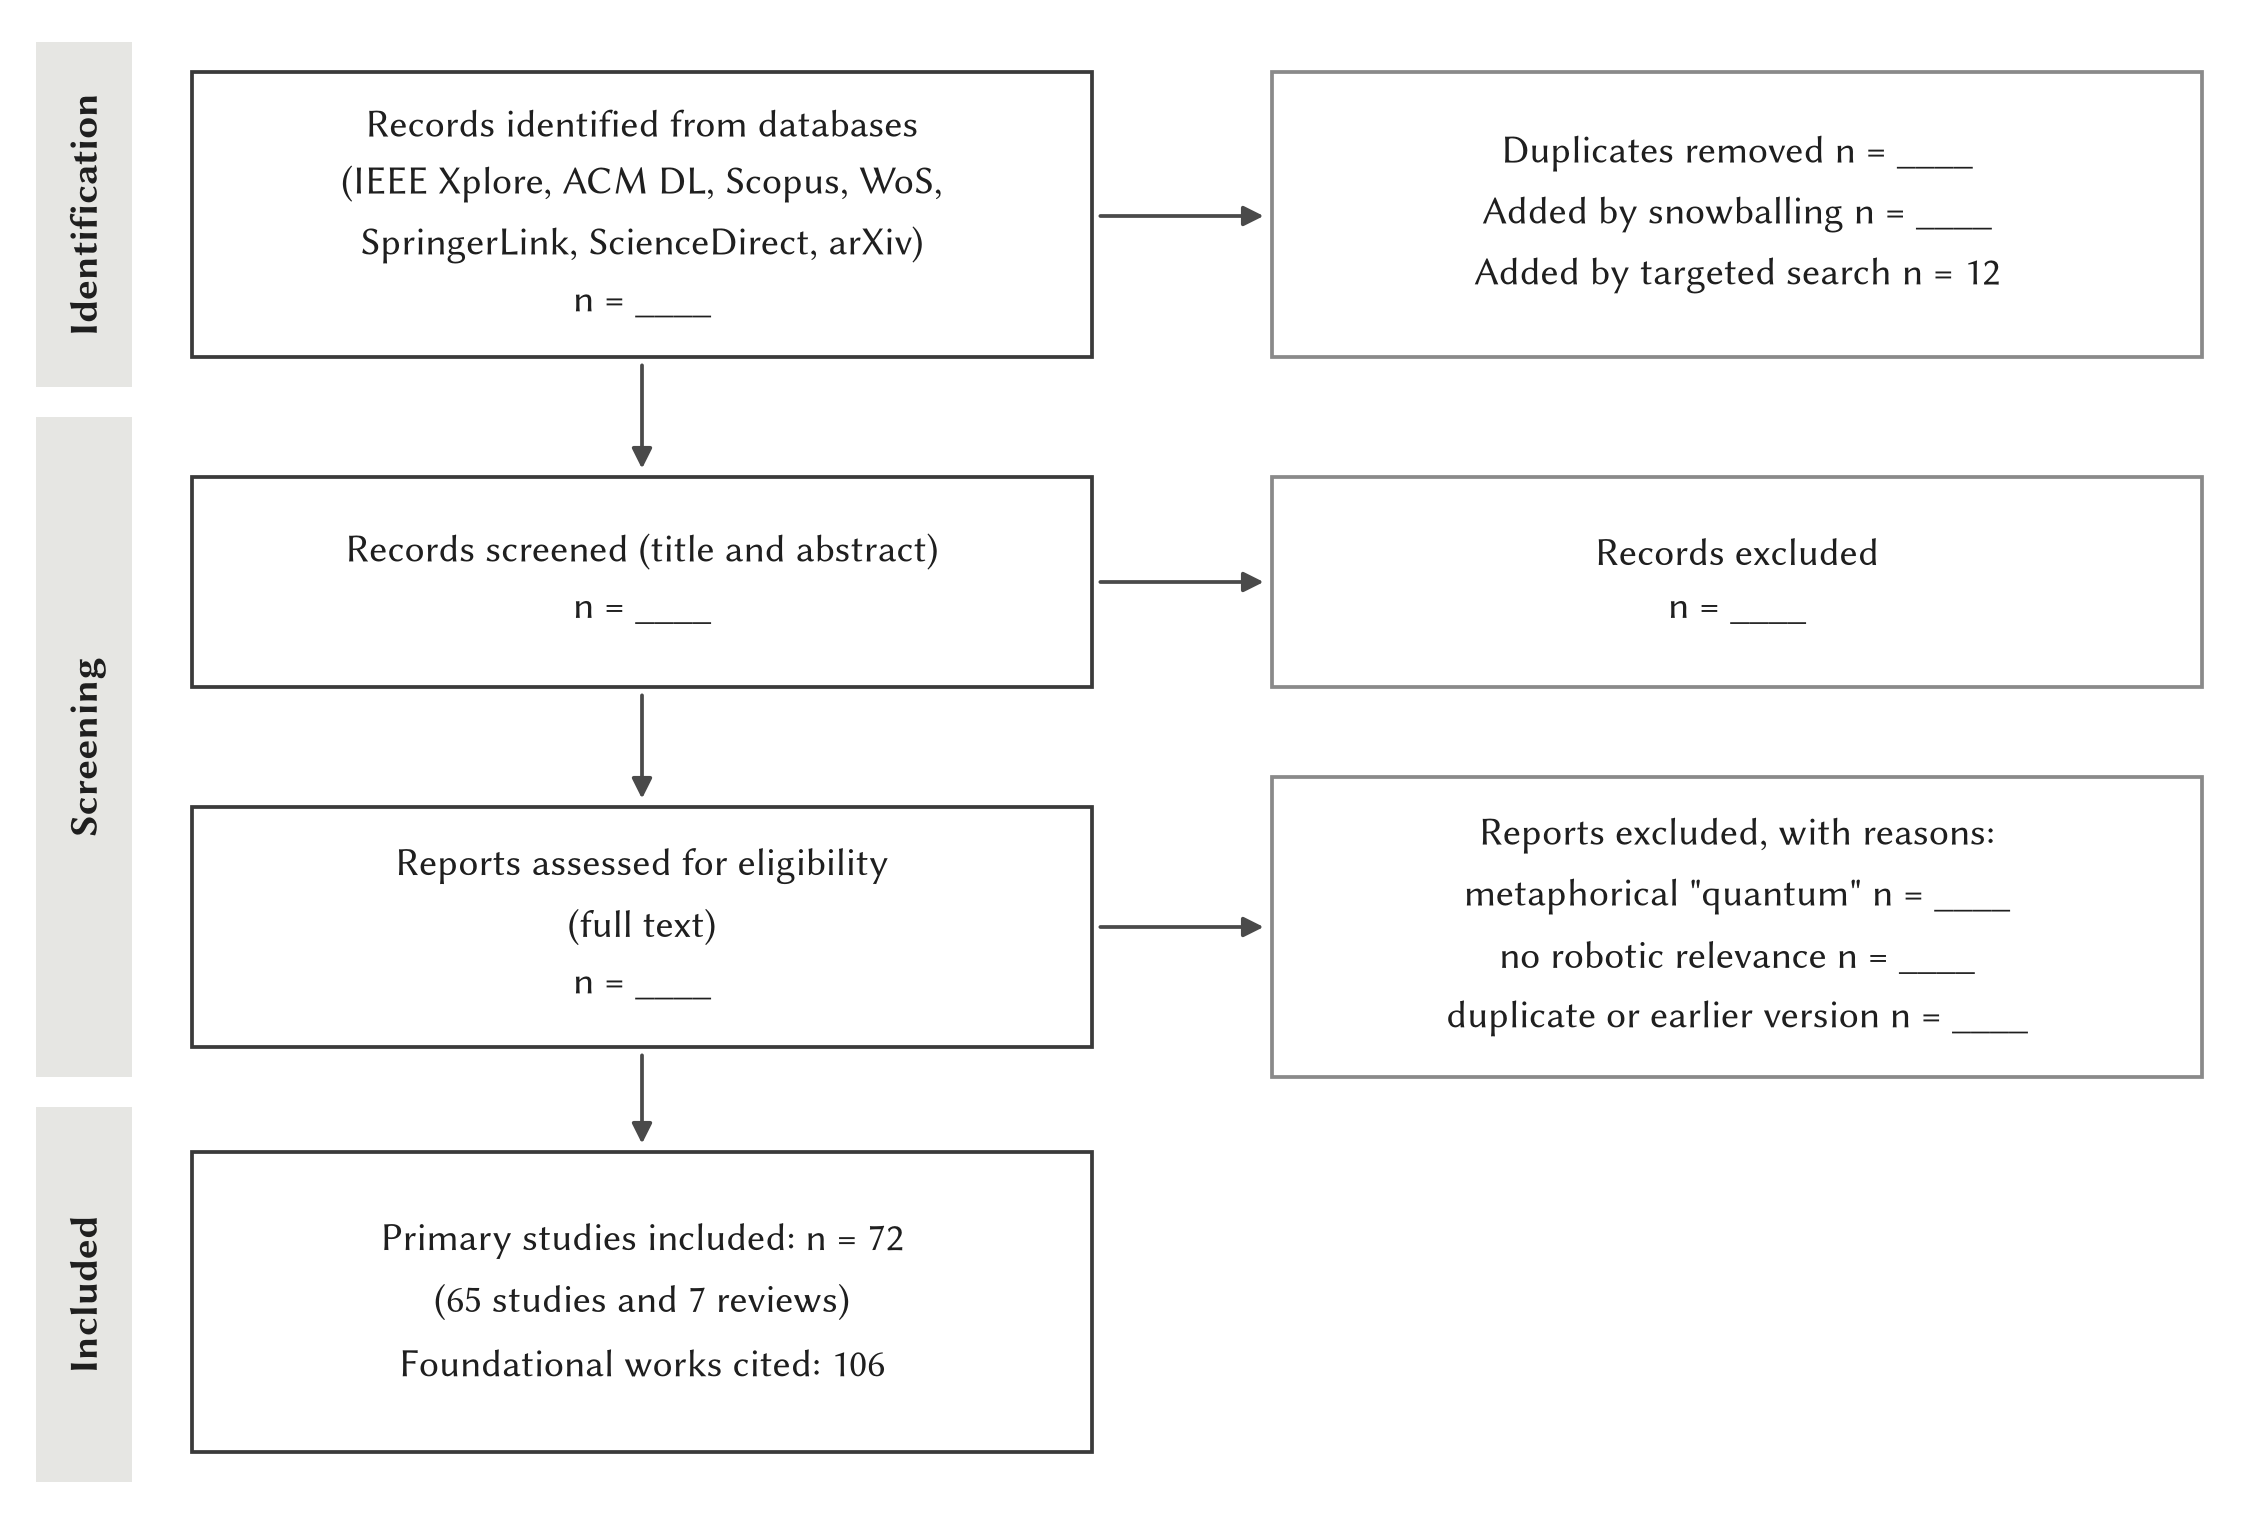
\includegraphics[width=0.8\linewidth]{figures/fig6_prisma.png}
\caption{PRISMA 2020 flow diagram. Stages for which the number of records was not logged are marked as such (see Table~\ref{tab:flow}).}
\Description{PRISMA 2020 flow diagram with boxes for identification, screening, eligibility, and inclusion, ending with 72 primary studies and 107 foundational works.}
\label{fig:prisma}
\end{figure}

\begin{table}[h]
\caption{PRISMA 2020 checklist: location of each item in the main article.}
\label{tab:prisma}
\footnotesize
\begin{tabular}{@{}>{\raggedright\arraybackslash}p{0.060\dimexpr\linewidth-6\tabcolsep\relax}>{\raggedright\arraybackslash}p{0.400\dimexpr\linewidth-6\tabcolsep\relax}>{\raggedright\arraybackslash}p{0.540\dimexpr\linewidth-6\tabcolsep\relax}@{}}
\toprule
\textbf{\#} & \textbf{Item} & \textbf{Location} \\ \midrule
1 & Title & Title \\
2 & Abstract & Abstract \\
3 & Rationale & Sections 1.1--1.3 \\
4 & Objectives & Section 3.1 (RQ1-RQ5) \\
5 & Eligibility criteria & Section 3.3 \\
6 & Information sources & Section 3.2; Table~\ref{tab:search} \\
7 & Search strategy & Table~\ref{tab:search} \\
8 & Selection process & Section 3.4 \\
9 & Data collection process & Section 3.5 \\
10 & Data items & Sections 3.5--3.6 \\
11 & Study risk of bias assessment & Section 3.5; criteria in Table~\ref{tab:rubric} \\
12 & Effect measures & Not applicable (no meta-analysis); evidence levels in Table 2 \\
13 & Synthesis methods & Sections 3.6 and 11 \\
14 & Reporting bias assessment & Section 3.7 \\
15 & Certainty assessment & Sections 11.2--11.3 \\
16 & Study selection & Figure S1 \\
17 & Study characteristics & Table S1 and the machine-readable evidence table \\
18 & Risk of bias in studies & Table~\ref{tab:appraisal}; Limitation column of Table S1; Sections 4--10 \\
19 & Results of individual studies & Sections 4--10; Table S1 \\
20 & Results of syntheses & Section 11; Tables 2 and 3 \\
21 & Reporting biases & Section 3.7 \\
22 & Certainty of evidence & Section 11.2 \\
23 & Discussion & Sections 11--12 \\
24 & Registration and protocol & The review protocol was not registered \\
25 & Support & This research received no external funding. It was carried out as part of the authors' work at Amrita Vishwa Vidyapeetham, Chennai, India. \\
26 & Competing interests & The authors declare no competing interests \\
27 & Availability of data, code, and materials & Table S1 and the machine-readable evidence table \\
\bottomrule
\end{tabular}
\end{table}

\begin{table}[h]
\caption{Quality-appraisal criteria for robotics application studies. Each criterion was judged as not met, partly met, or met; the judgments were not summed into a score, and the criteria a study does not meet are reported in the Limitation column of Table S1.}
\label{tab:rubric}
\footnotesize
\begin{tabular}{@{}>{\raggedright\arraybackslash}p{0.250\dimexpr\linewidth-8\tabcolsep\relax}>{\raggedright\arraybackslash}p{0.220\dimexpr\linewidth-8\tabcolsep\relax}>{\raggedright\arraybackslash}p{0.260\dimexpr\linewidth-8\tabcolsep\relax}>{\raggedright\arraybackslash}p{0.270\dimexpr\linewidth-8\tabcolsep\relax}@{}}
\toprule
\textbf{Criterion} & \textbf{Not met} & \textbf{Partly met} & \textbf{Met} \\ \midrule
Q1 Problem formulation & Robotic task unclear & Task stated but simplified without justification & Task and mapping to the quantum formulation fully specified \\
Q2 Classical baseline & None & Basic or untuned baseline & State-of-the-art, tuned baseline \\
Q3 Experimental realism & Theory or toy example & Simulation or small QPU run & Physical robot or realistic field setting \\
Q4 Hardware and noise reporting & Not reported & Partly reported & Device, qubits, shots, noise, and mitigation reported \\
Q5 Performance metrics & Qualitative only & Task metric only & Task metric plus runtime, latency, or resources \\
Q6 Reproducibility & No details & Partial parameters & Code and data or full parameters available \\
Q7 Critical discussion & Absent & Brief & Explicit limitations and threats to validity \\
\bottomrule
\end{tabular}
\end{table}


{\footnotesize
\begin{longtable}{@{}>{\raggedright\arraybackslash}p{0.300\dimexpr\linewidth-14\tabcolsep\relax}>{\centering\arraybackslash}p{0.100\dimexpr\linewidth-14\tabcolsep\relax}>{\centering\arraybackslash}p{0.100\dimexpr\linewidth-14\tabcolsep\relax}>{\centering\arraybackslash}p{0.100\dimexpr\linewidth-14\tabcolsep\relax}>{\centering\arraybackslash}p{0.100\dimexpr\linewidth-14\tabcolsep\relax}>{\centering\arraybackslash}p{0.100\dimexpr\linewidth-14\tabcolsep\relax}>{\centering\arraybackslash}p{0.100\dimexpr\linewidth-14\tabcolsep\relax}>{\centering\arraybackslash}p{0.100\dimexpr\linewidth-14\tabcolsep\relax}@{}}
\caption{Quality appraisal of the 59 graded application studies (the six purely theoretical L1 studies and the seven reviews are not appraised) against the criteria of Table~\ref{tab:rubric}. M = met, P = partly met, N = not met; n/a = not applicable (quantum-inspired algorithms on classical hardware). \fillin{Q4 and Q6 for the 3 studies marked [ ] to be completed once their full texts are obtained}.}\label{tab:appraisal}\\
\toprule
\textbf{Study} & \textbf{Q1} & \textbf{Q2} & \textbf{Q3} & \textbf{Q4} & \textbf{Q5} & \textbf{Q6} & \textbf{Q7} \\ \midrule
\endfirsthead
\toprule
\textbf{Study} & \textbf{Q1} & \textbf{Q2} & \textbf{Q3} & \textbf{Q4} & \textbf{Q5} & \textbf{Q6} & \textbf{Q7} \\ \midrule
\endhead
\citet{Dong2006} & P & N & P & N & P & P & P \\
\citet{Ohzeki2019} & M & M & P & P & M & P & M \\
\citet{Quang2025} & M & P & P & P & M & P & P \\
\citet{Clark2019} & M & P & P & P & P & M & P \\
\citet{Smierzchalski2024} & M & M & P & P & M & M & M \\
\citet{Leib2023} & M & M & P & P & M & P & M \\
\citet{AtchadeAdelomou2021} & M & N & P & P & P & P & P \\
\citet{Windmann2023} & M & N & P & \fillin{} & M & \fillin{} & P \\
\citet{Schuetz2022} & M & M & P & P & M & P & M \\
\citet{Willmann2025} & M & M & P & P & M & P & M \\
\citet{Osaba2025} & M & M & P & P & P & M & P \\
\citet{Otani2025} & M & N & P & P & P & P & P \\
\citet{Salloum2026} & M & P & P & M & M & P & M \\
\citet{Wang2025} & M & P & P & P & P & M & P \\
\citet{Roh2025} & M & P & P & P & P & P & P \\
\citet{Goncalves2018} & P & N & N & M & P & P & P \\
\citet{Dong2012} & M & P & M & n/a & P & P & P \\
\citet{Hohenfeld2024} & M & M & P & P & P & M & M \\
\citet{Dragan2025} & M & M & P & P & P & P & M \\
\citet{Sinha2023} & M & P & P & M & P & M & P \\
\citet{Acuto2022} & M & M & P & P & P & P & P \\
\citet{Lokossou2025} & M & P & P & P & P & P & P \\
\citet{Altrabulsi2026} & M & P & P & M & P & M & P \\
\citet{Taghavi2025} & P & P & P & P & P & M & P \\
\citet{Park2023} & M & P & P & P & P & P & P \\
\citet{Park2024} & P & P & P & P & P & P & P \\
\citet{Sun2025} & M & N & M & P & M & P & M \\
\citet{Ngo2026} & M & N & P & M & M & P & M \\
\citet{Chella2022} & M & N & P & P & P & P & P \\
\citet{Chella2023} & M & P & P & P & P & M & P \\
\citet{Lathrop2023} & M & P & P & P & P & M & P \\
\citet{Nigatu2025} & M & P & P & M & P & P & P \\
\citet{Sarkar2024} & M & M & P & P & P & P & P \\
\citet{Gerlach2025} & M & M & P & P & M & P & M \\
\citet{Innan2025} & M & N & P & M & P & P & P \\
\citet{OsabaDrone2025} & M & N & P & P & P & P & P \\
\citet{Bang2026} & M & N & P & P & P & P & P \\
\citet{Rao2024} & M & P & P & P & P & P & P \\
\citet{GonzalezVillasmil2026} & M & P & P & P & M & M & M \\
\citet{Yu2025} & M & P & P & P & P & P & P \\
\citet{Antero2025} & M & P & P & M & P & P & P \\
\citet{Cheiney2018} & M & P & P & M & M & P & P \\
\citet{Templier2022} & M & P & P & M & M & P & P \\
\citet{Wang2021} & M & P & P & P & P & P & P \\
\citet{Wang2023} & M & P & P & P & P & P & P \\
\citet{Muradoglu2025} & M & M & M & P & M & P & P \\
\citet{Khoshnoud2020} & P & N & P & N & N & N & P \\
\citet{Tian2023} & M & N & M & P & M & P & P \\
\citet{Liu2021} & M & N & M & M & M & P & P \\
\citet{Conrad2025} & M & N & M & M & M & M & M \\
\citet{Widdows2023} & M & N & P & P & P & P & M \\
\citet{Yan2021} & P & N & P & N & P & N & P \\
\citet{Daglarli2025} & P & P & P & P & P & P & P \\
\citet{Essalmi2026} & M & P & P & P & P & P & P \\
\citet{Zuo2018} & M & P & P & n/a & P & P & P \\
\citet{Fazilat2025b} & M & P & P & n/a & P & M & P \\
\citet{Mannone2022} & P & N & N & P & N & M & P \\
\citet{Mannone2023} & P & N & P & \fillin{} & P & \fillin{} & M \\
\citet{Mannone2025} & M & P & P & \fillin{} & P & \fillin{} & M \\
\bottomrule
\end{longtable}}

\begin{table}[h]
\caption{Databases and search strings.}
\label{tab:search}
\footnotesize
\begin{tabular}{@{}>{\raggedright\arraybackslash}p{0.220\dimexpr\linewidth-4\tabcolsep\relax}>{\raggedright\arraybackslash}p{0.780\dimexpr\linewidth-4\tabcolsep\relax}@{}}
\toprule
\textbf{Database or field} & \textbf{Search string (adapted to each database syntax)} \\ \midrule
Core string & (``quantum computing'' OR ``quantum algorithm*'' OR ``quantum annealing'' OR QAOA OR ``variational quantum'' OR ``quantum machine learning'' OR ``quantum reinforcement learning'' OR ``quantum-inspired'' OR ``quantum sensing'' OR ``quantum cognition'' OR ``quantum probability'') AND (robot* OR ``autonomous vehicle*'' OR ``mobile robot*'' OR swarm OR UAV OR AGV OR manipulator) AND (planning OR navigation OR localization OR ``path planning'' OR ``task allocation'' OR routing OR control OR learning OR ``decision making'' OR SLAM OR kinematics) \\
Foundations string & (``quantum computing'' OR ``quantum algorithm*'') AND (review OR survey OR tutorial) AND (NISQ OR ``error mitigation'' OR ``barren plateau*'' OR ``fault-tolerant'' OR dequantiz*) \\
IEEE Xplore & Core string in All Metadata; 1982 to October 2026 \\
ACM Digital Library & Core string in Title, Abstract, Keywords \\
Scopus & TITLE-ABS-KEY(core string) \\
Web of Science & TS=(core string) \\
SpringerLink, ScienceDirect & Core string in full text, restricted to articles and conference papers \\
arXiv & Categories quant-ph, cs.RO, cs.LG; title and abstract terms from the core string \\
Snowballing & Backward and forward citation search from \citet{Petschnigg2019}, \citet{Yan2024}, \citet{Meyer2022}, and \citet{Tandon2017} \\
Targeted search & Drones and UAVs, multi-agent and autonomous mobility, autonomous driving, control benchmarks (cart-pole), and automated storage and retrieval, each combined with the quantum block of the core string; 12 additional primary studies \\
\bottomrule
\end{tabular}
\end{table}

\clearpage
\section*{Method Schematics, Synthesis Table, Reporting Checklist, and Roadmap}
The following figures and tables accompany Sections 4--6, 9, 11, and 12 of the main article.

\begin{figure}[p]
\centering
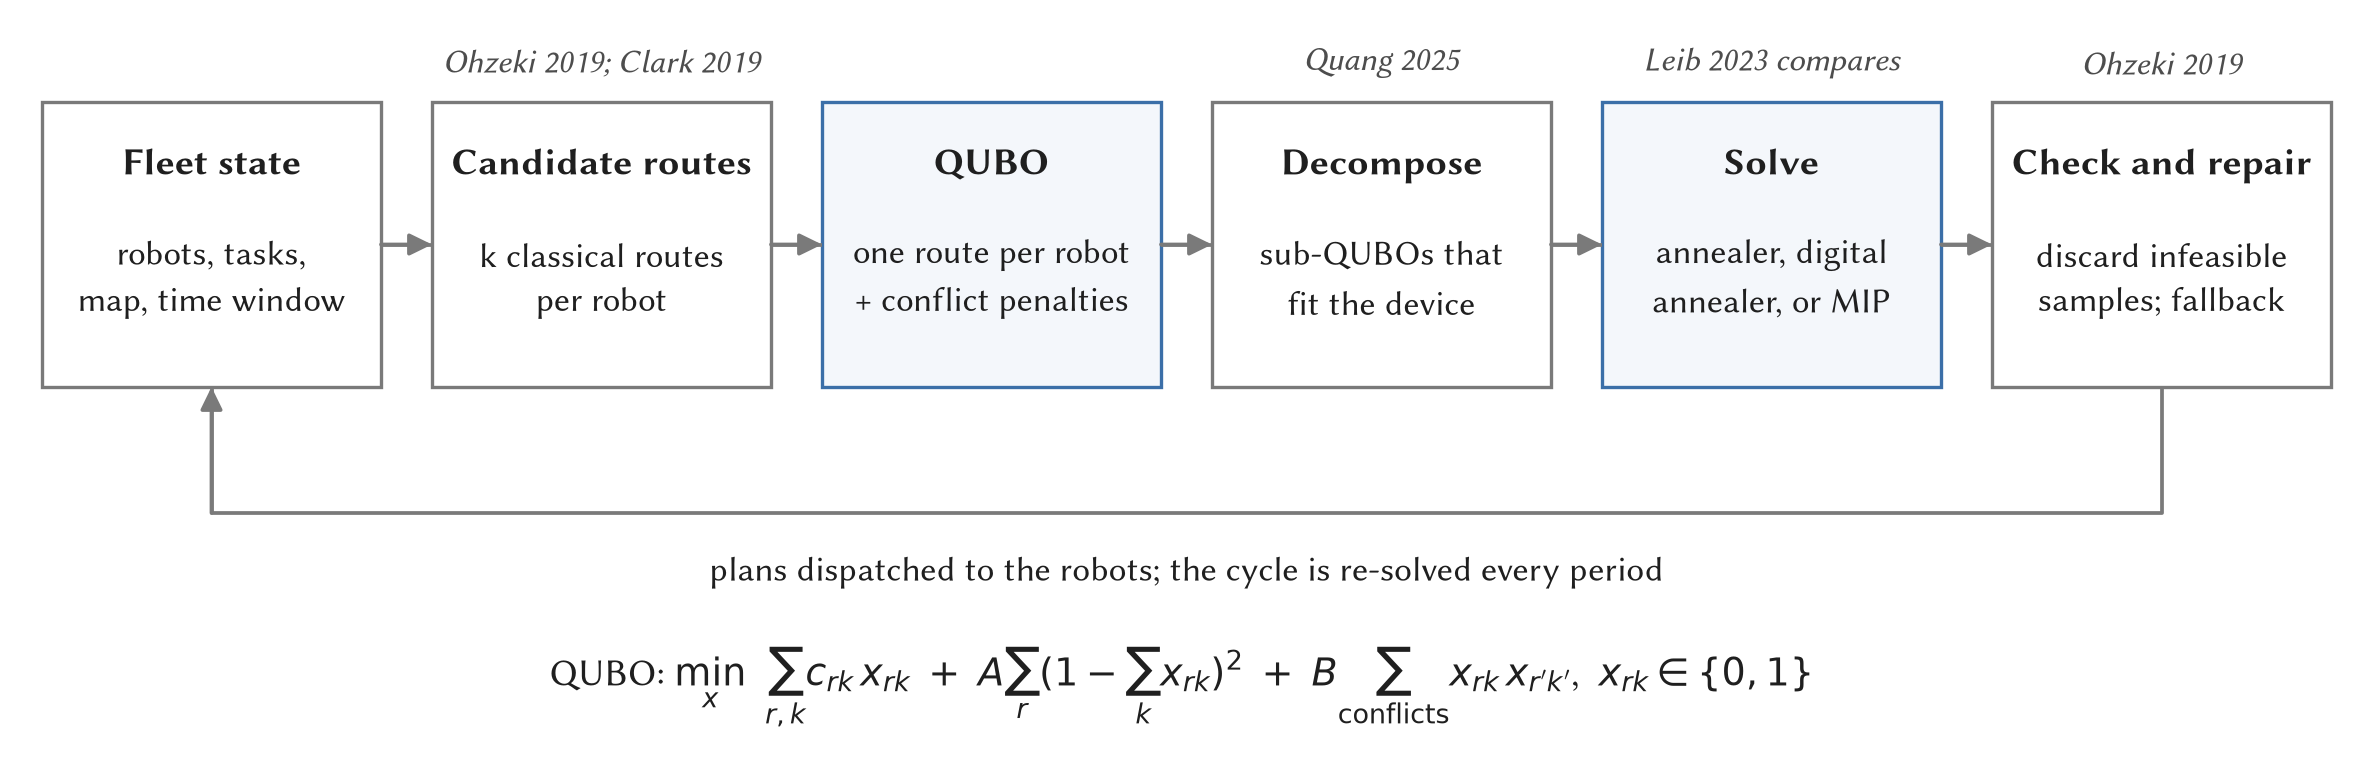
\includegraphics[width=\linewidth]{figures/fig8_qubo_pipeline.png}
\caption{The annealing pipeline shared by the fleet-routing studies. Each vehicle selects one route from a candidate set, penalty terms forbid double selection and conflicting road use, large instances are decomposed, and returned samples are checked and repaired before dispatch; the loop repeats in every planning period. Redrawn and generalized from the formulations of \citet{Ohzeki2019}, \citet{Clark2019}, and \citet{Quang2025}, with the solver comparison of \citet{Leib2023}.}
\Description{Flow diagram with six boxes from left to right: fleet state, candidate routes, QUBO with one-route and conflict penalties, decomposition into subproblems, solving on an annealer or classical solver, and check and repair. A feedback arrow returns from the last box to the first for the next planning period. Short notes above each box name the studies that use that step.}
\label{fig:qubo}
\end{figure}

\begin{figure}[p]
\centering
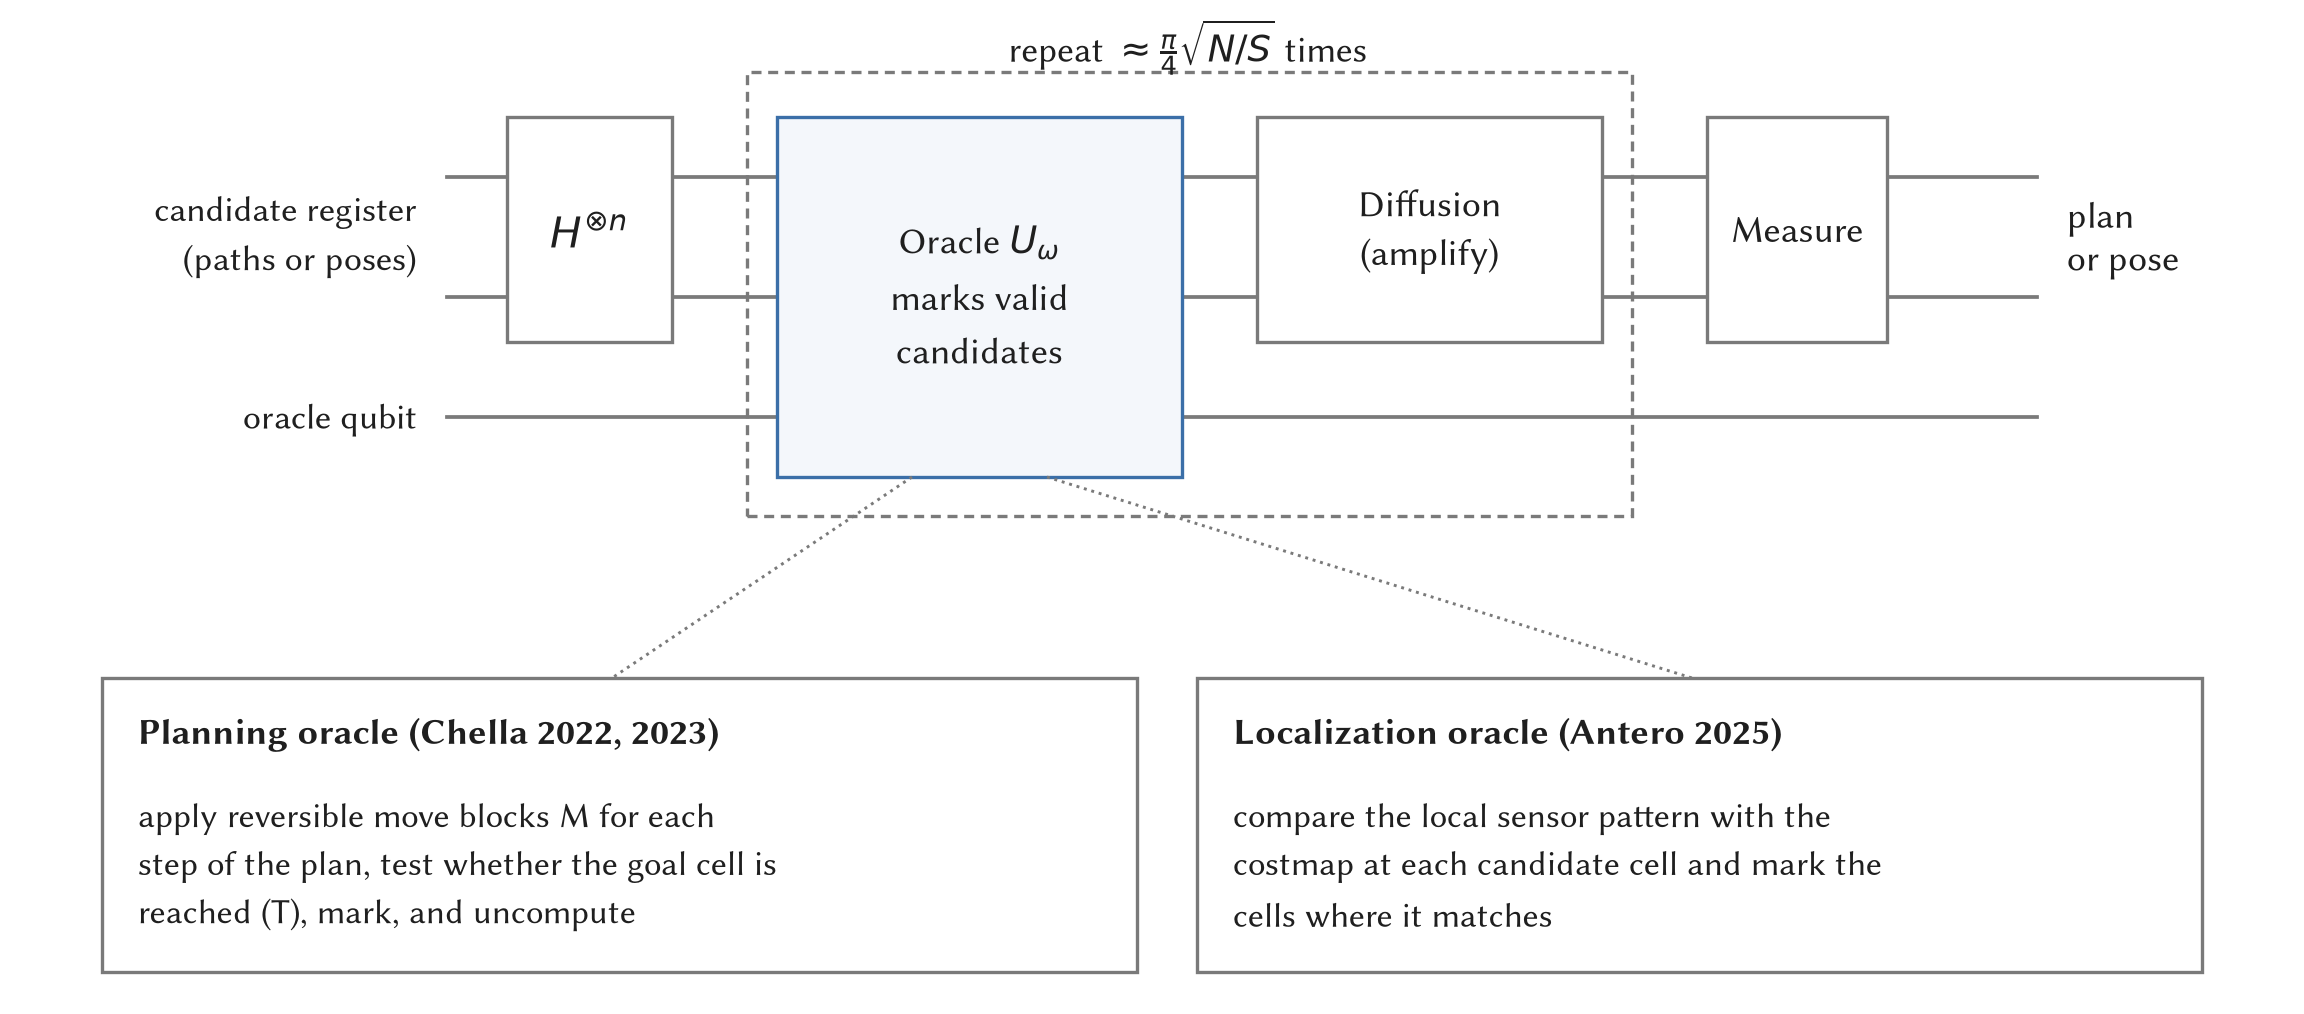
\includegraphics[width=\linewidth]{figures/fig9_grover.png}
\caption{Grover search as used for robot planning and localization. After a uniform superposition, the oracle marks goal-reaching action sequences \citep{Chella2022,Chella2023} or map cells whose stored pattern matches the current sensor view \citep{Antero2025}, and the diffusion step amplifies the marked states; about $\frac{\pi}{4}\sqrt{N/S}$ repetitions are needed for $N$ candidates and $S$ solutions. Redrawn from the circuit descriptions in those studies.}
\Description{Circuit-style diagram: Hadamard gates on n qubits, then an oracle and a diffusion operator inside a dashed box repeated about pi over four times the square root of N over S, then measurement. Two panels below describe the planning oracle, which marks action sequences that reach the goal, and the localization oracle, which marks map cells matching the sensor pattern.}
\label{fig:grover}
\end{figure}

\begin{figure}[p]
\centering
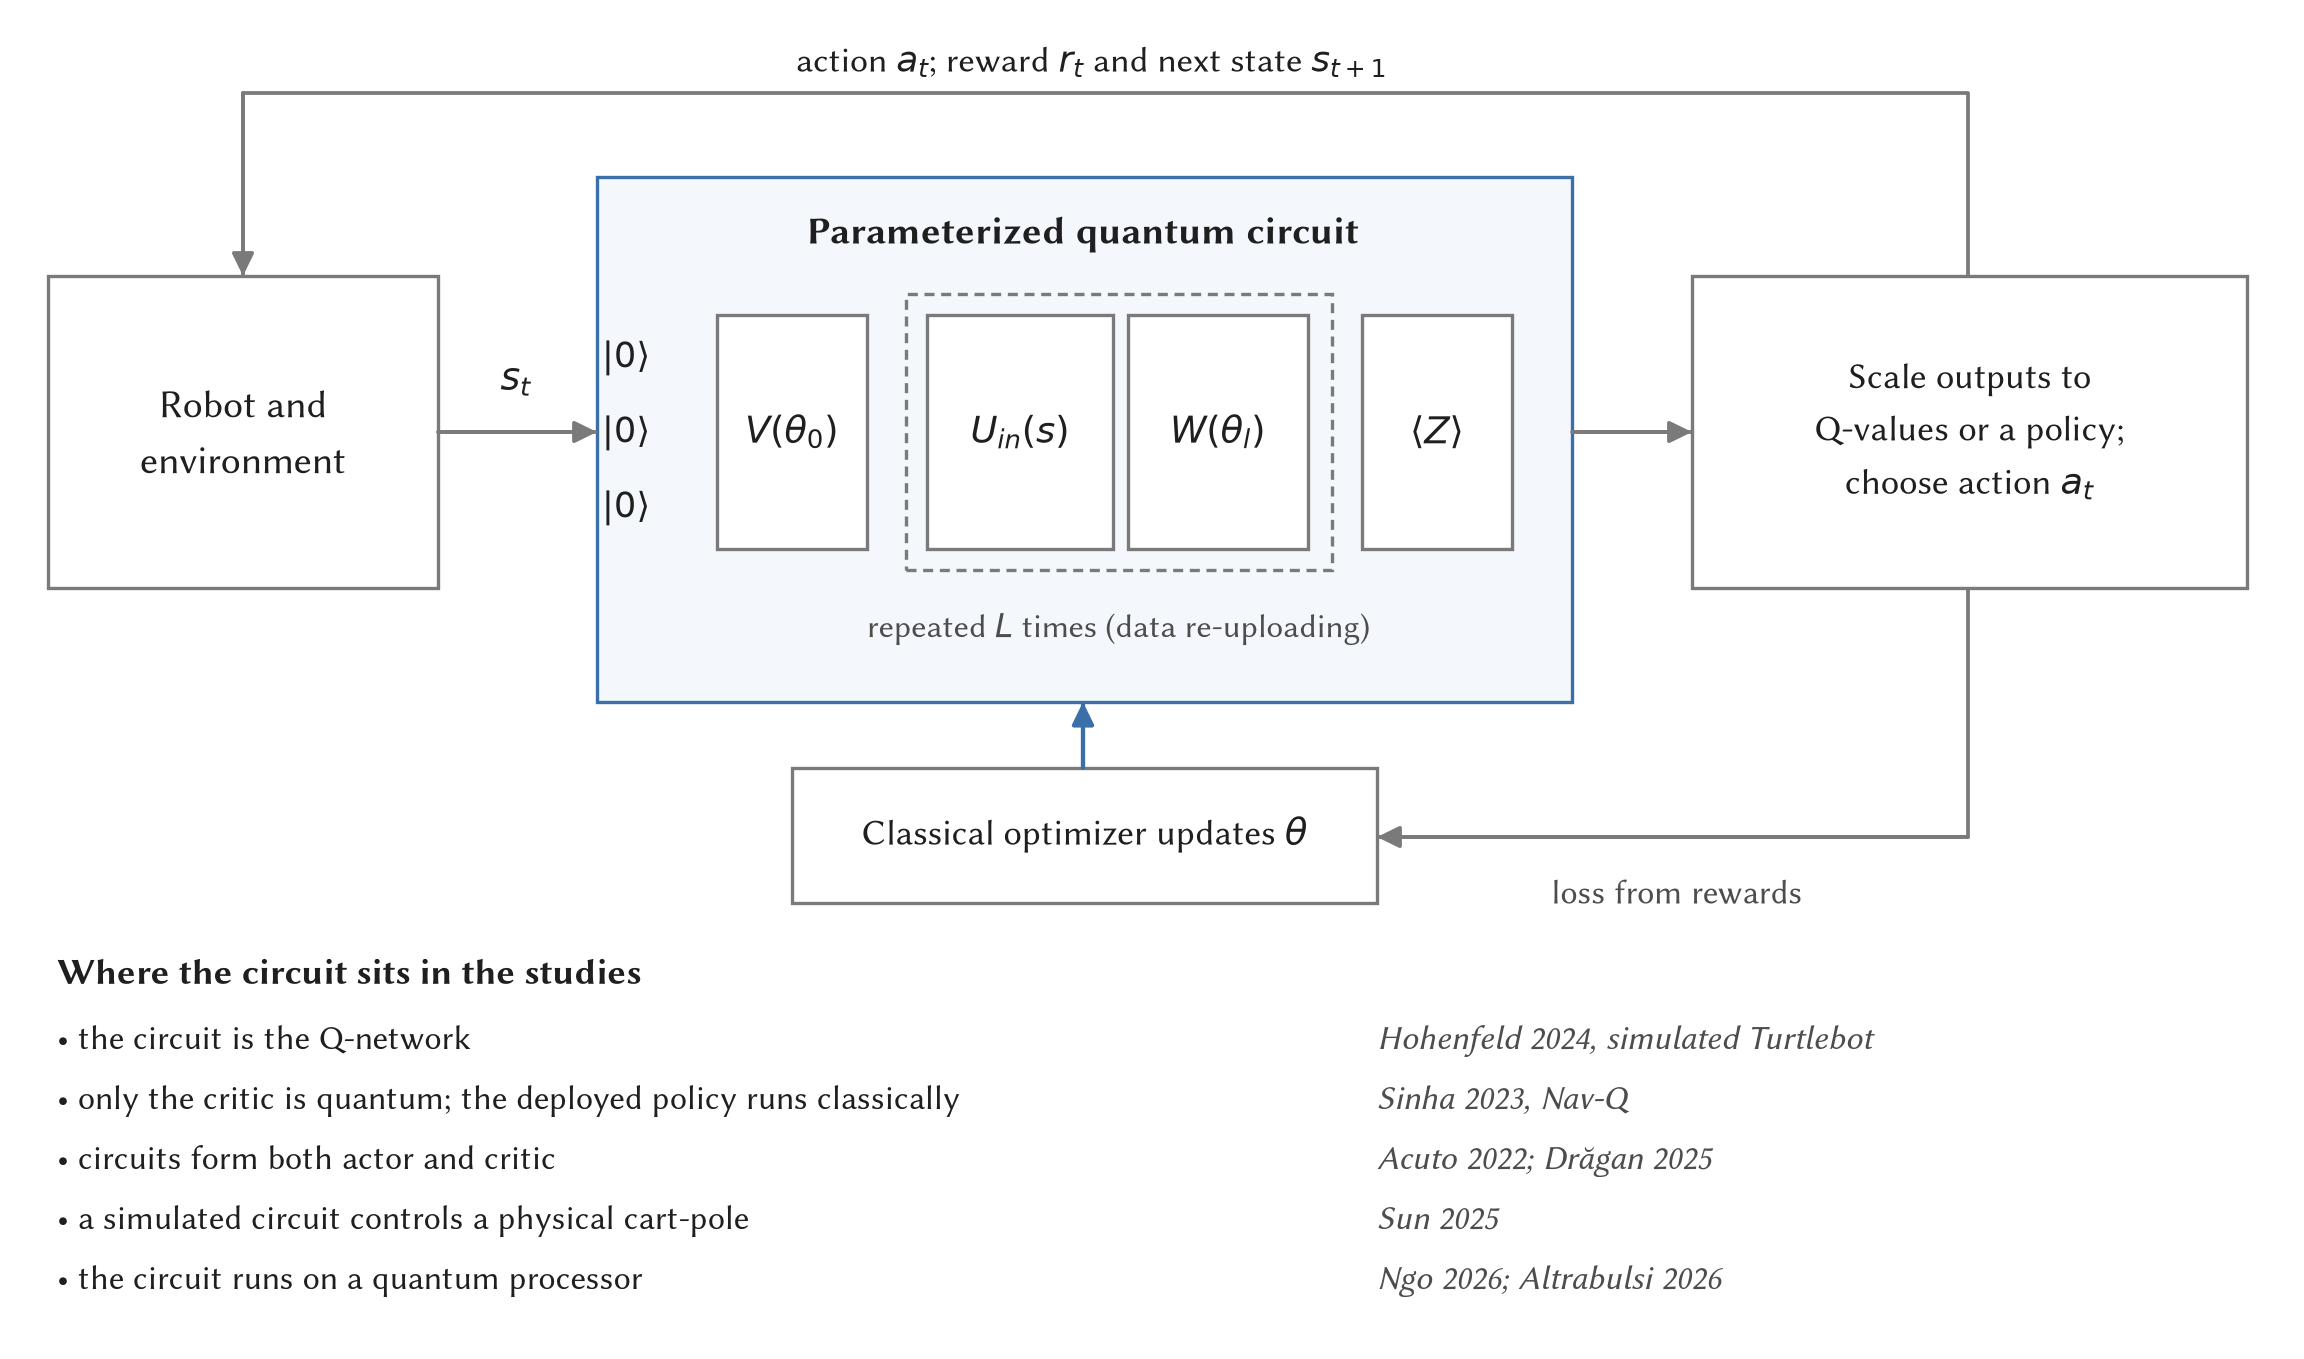
\includegraphics[width=\linewidth]{figures/fig10_vqc_policy.png}
\caption{The variational policy template common to the quantum reinforcement-learning studies: the robot state is encoded by data re-uploading, trainable layers are repeated $L$ times, measured expectation values are scaled into actions or values, and a classical optimizer updates the parameters. Adapted from the architectures of \citet{Hohenfeld2024}, \citet{Sinha2023}, \citet{Acuto2022}, \citet{Dragan2025}, \citet{Sun2025}, \citet{Ngo2026}, and \citet{Altrabulsi2026}; the list on the right notes where the circuit sits in each study.}
\Description{Diagram of a robot sending its state to a parameterized quantum circuit made of an initial layer, a dashed block of encoding and trainable layers repeated L times, and Pauli-Z measurements. The outputs are scaled into actions sent back to the robot, and a classical optimizer loop updates the circuit parameters. A side list names the studies and whether the circuit acts as policy, critic, or onboard controller.}
\label{fig:vqc}
\end{figure}

\begin{figure}[p]
\centering
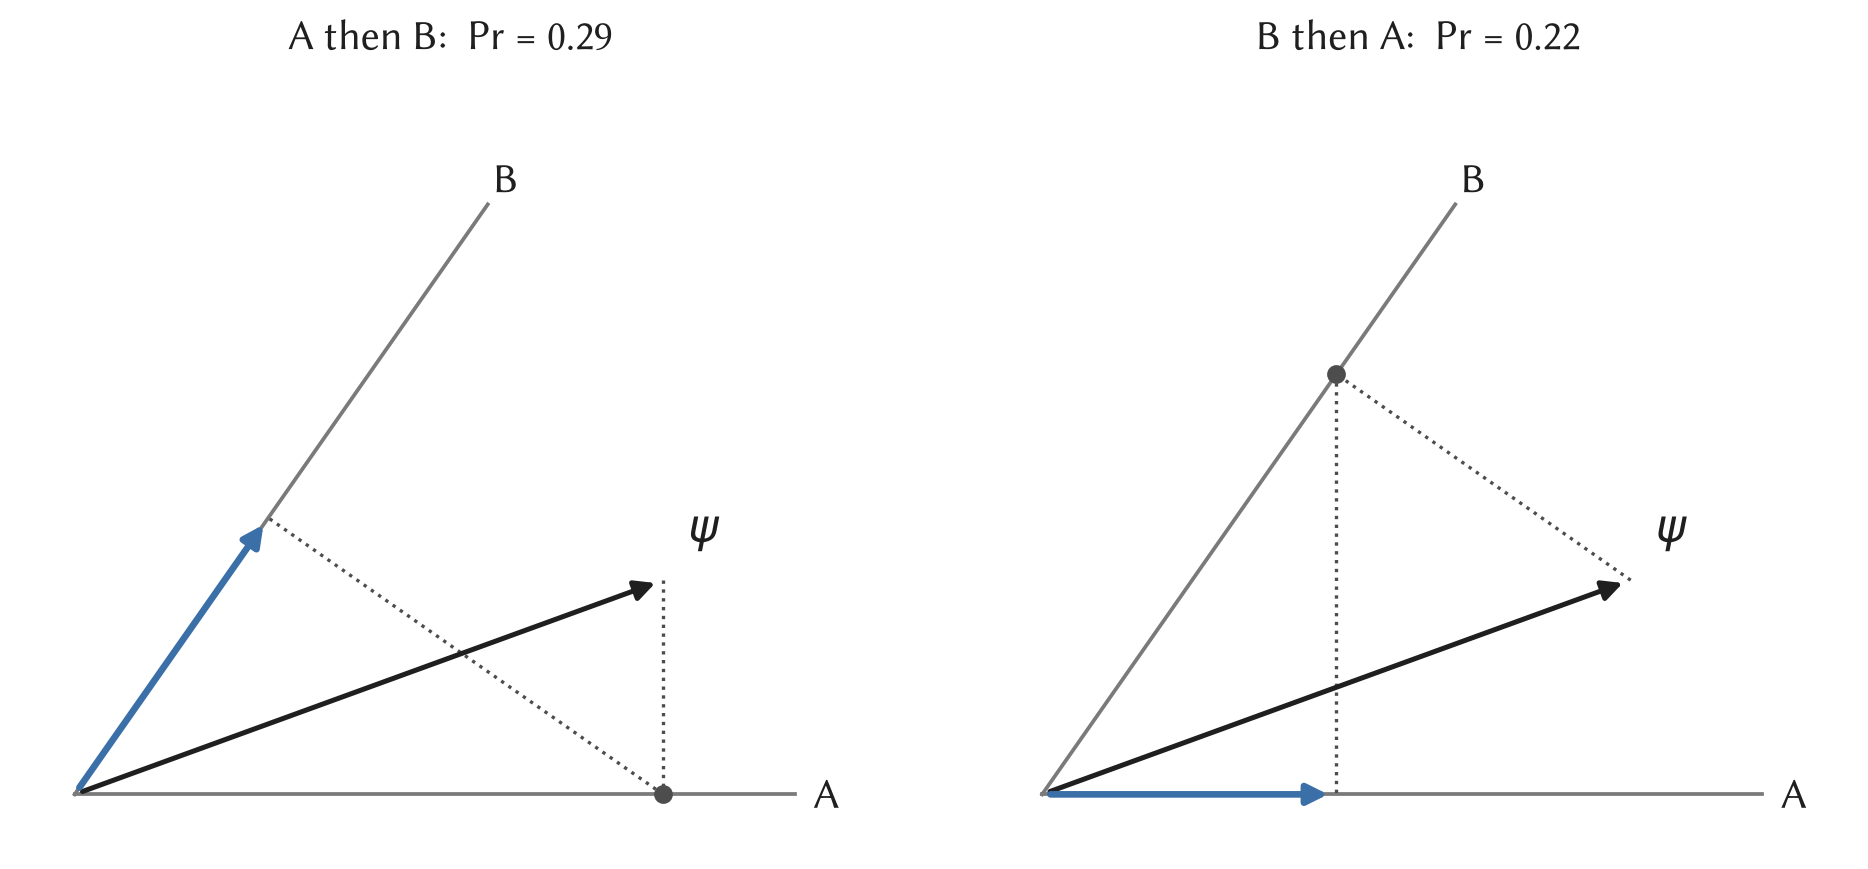
\includegraphics[width=0.92\linewidth]{figures/fig11_order_effect.png}
\caption{Why the order of questions matters in quantum probability. A belief state $\psi$ is projected first onto one answer subspace and then onto the other; because the projectors do not commute, the probability of answering yes to both depends on the order. The angles ($\psi=20^\circ$, $A=0^\circ$, $B=55^\circ$) are illustrative. Adapted from the geometric account of \citet{Busemeyer2012} and \citet{Pothos2013}, which \citet{Widdows2023} implemented as single-qubit circuits.}
\Description{Two panels with a unit circle. The left panel projects the state onto axis A and then onto axis B, giving probability 0.29; the right panel projects onto B first and then onto A, giving probability 0.22.}
\label{fig:order}
\end{figure}

\begin{table}[p]
\caption{Cross-domain synthesis of quantum and quantum-inspired methods for robotics. Evidence levels follow Table 2 of the main article; ``sim.'' denotes a simulated robot environment.}
\label{tab:synthesis}
\footnotesize
\begin{tabular}{@{}>{\raggedright\arraybackslash}p{0.270\dimexpr\linewidth-10\tabcolsep\relax}>{\raggedright\arraybackslash}p{0.210\dimexpr\linewidth-10\tabcolsep\relax}>{\raggedright\arraybackslash}p{0.100\dimexpr\linewidth-10\tabcolsep\relax}>{\raggedright\arraybackslash}p{0.240\dimexpr\linewidth-10\tabcolsep\relax}>{\raggedright\arraybackslash}p{0.180\dimexpr\linewidth-10\tabcolsep\relax}@{}}
\toprule
\textbf{Application} & \textbf{Quantum method} & \textbf{Evidence} & \textbf{Current limitation} & \textbf{Deployment potential} \\ \midrule
Fleet and multi-robot routing, AGV and storage-system scheduling~\cite{Ohzeki2019,Clark2019,Quang2025,Smierzchalski2024,Leib2023,Windmann2023} & QUBO with quantum annealing or hybrid solvers & L3--L4 (sim.) & Decomposition needed; classical and digital annealers competitive or better & Medium: periodic, offline \\
Multi-agent pathfinding~\cite{Gerlach2025,GonzalezVillasmil2026} & QUBO subproblems in exact classical framework & L2--L3 & Small QUBOs; structure-dependent & Medium \\
Industrial trajectories, assembly, inspection~\cite{Schuetz2022,Willmann2025,Osaba2025} & QUBO and annealing in classical pipelines & L3 & Classical algorithm does most of the work; overheads & Low-medium \\
Warehouse picking~\cite{AtchadeAdelomou2021} & QUBO with VQE and QAOA via cloud & L3 & Tiny instances; cloud latency & Low-medium \\
Inverse kinematics~\cite{Otani2025,Salloum2026,Nigatu2025} & Gate-based VQA, annealing, QML with Grover & L2--L3 & Toy size; continuous classical IK solvers stronger & Low \\
Motion and swarm planning~\cite{Benioff2002,Chella2022,Chella2023,Lathrop2023} & Grover search & L1--L2 & Oracle depth; noiseless simulation & Low (needs fault tolerance) \\
UAV path, routing, and task assignment; view planning~\cite{Innan2025,Yu2025,Sarkar2024,OsabaDrone2025,Bang2026} & QAOA, annealing, variational, hybrid quantum ACO & L2--L3 & Small graphs; weak baselines & Low-medium \\
Localization~\cite{Antero2025} & Grover pattern search & L3 & Noise; simulation limited to about 40 qubits & Low (needs fault tolerance) \\
Navigation, locomotion, and multi-agent RL~\cite{Hohenfeld2024,Dragan2025,Altrabulsi2026,Lokossou2025,Taghavi2025,Park2023,Park2024} & VQC-based deep RL & L3--L4 (sim.) & No advantage over adequately sized classical networks & Medium: compact embedded policies \\
Driving and arm control~\cite{Sinha2023,Acuto2022} & Quantum critic; variational SAC & L4 (sim.) & Simulation only & Medium (training-time use) \\
Real-time control (cart-pole)~\cite{Sun2025,Ngo2026} & Variational policies; QPU inference & L3--L5 & Toy system; cloud QPU too slow; simulated circuit on hardware & Medium (shows latency limits) \\
Object detection for driving~\cite{Roh2025} & Quantum CNN & L2 & Simulated circuits & Low-medium \\
Navigation, SLAM, IK (quantum-inspired)~\cite{Dong2012,Zuo2018,Fazilat2025b} & QiRL, QPSO, quantum-inspired networks & L2--L5 & Weak baselines & High (runs classically today) \\
GNSS-denied navigation~\cite{Muradoglu2025,Cheiney2018,Templier2022} & Quantum magnetometers, atom interferometers & L3--L6 & SWaP-C, bandwidth & High (near-term) \\
Human decision modeling, HRI, human-machine teams, driving interaction~\cite{Widdows2023,Yan2021,Lawless2023,Humr2025,Essalmi2026} & Quantum-probability models & L1--L3 & No HRI evaluation yet & Medium-high (hardware-light; untested on robots) \\
Swarms and distributed robots~\cite{Mannone2023,Mannone2025} & Pairwise quantum circuits & L3--L4 (sim.) & QPU access at every interaction & Low \\
Secure robot and drone communication~\cite{Tian2023,Conrad2025,Khoshnoud2020,Liu2021} & QKD, photonic hardware & L5 & Range, SWaP, weather & High (security, near-term) \\
\bottomrule
\end{tabular}
\end{table}

\begin{table}[p]
\caption{Proposed minimal reporting checklist for quantum-robotics experiments.}
\label{tab:checklist}
\footnotesize
\begin{tabular}{@{}>{\raggedright\arraybackslash}p{0.240\dimexpr\linewidth-4\tabcolsep\relax}>{\raggedright\arraybackslash}p{0.760\dimexpr\linewidth-4\tabcolsep\relax}@{}}
\toprule
\textbf{Item} & \textbf{What to report} \\ \midrule
1. Task and formulation & Robotic task, its mapping to the quantum formulation (e.g., QUBO size, penalty weights, encoding), and any discretization relative to the original continuous problem. \\
2. Quantum type & Genuinely quantum or quantum-inspired; quantum hardware, simulator, or digital annealer used; noise model for simulations. \\
3. Classical baseline & State-of-the-art, tuned classical method (e.g., Gurobi, CPLEX, RRT*, A*, adequately sized deep RL) with comparable resources. \\
4. Quantum resources & Qubits, circuit depth, two-qubit gate count, shots, optimizer iterations, embedding size, and error-mitigation method. \\
5. End-to-end time and energy & Wall-clock time including queueing, compilation or embedding, and post-processing; energy where possible. \\
6. Task metrics & Success rate, solution quality, path length, or error, with variance over seeds or instances. \\
7. Evidence level & Level reached in Table 2 of the main article, and whether the quantum component runs in the real-time loop. \\
8. Reproducibility & Code, data, hyperparameters, device name, and calibration date. \\
\bottomrule
\end{tabular}
\end{table}

\begin{table}[p]
\caption{Research agenda derived from the taxonomy, arranged by time horizon.}
\label{tab:roadmap}
\footnotesize
\begin{tabular}{@{}>{\raggedright\arraybackslash}p{0.130\dimexpr\linewidth-8\tabcolsep\relax}>{\raggedright\arraybackslash}p{0.500\dimexpr\linewidth-8\tabcolsep\relax}>{\raggedright\arraybackslash}p{0.150\dimexpr\linewidth-8\tabcolsep\relax}>{\raggedright\arraybackslash}p{0.220\dimexpr\linewidth-8\tabcolsep\relax}@{}}
\toprule
\textbf{Horizon} & \textbf{Research direction} & \textbf{Function} & \textbf{Key references} \\ \midrule
Near term (1--3 years) & Integrate quantum magnetometers and cold-atom accelerometers into robot navigation stacks with Kalman-type fusion and independent field validation & Sensing & \cite{Muradoglu2025,Cheiney2018} \\
 & Develop QP decision and human-modeling modules for social and collaborative robots; evaluate them with human participants against Bayesian and POMDP baselines & Decision-making & \cite{Pothos2022,Kurniawati2022} \\
 & Establish benchmarks and reporting standards (Table \ref{tab:checklist}) & All & - \\
 & Use quantum and quantum-inspired QUBO solvers for offline and periodic fleet optimization with classical fallbacks & Optimization & \cite{Quang2025,Gerlach2025,Goto2019} \\
 & Evaluate QKD for secure multi-robot and drone communication & Communication & \cite{Conrad2025} \\
Medium term (3--5 years) & Train QRL policies on real QPUs where parameter efficiency matters for embedded deployment, and test for sample-efficiency gains on physical robots & Learning & \cite{Hohenfeld2024,Kober2013} \\
 & Build edge (on-premise) QPU architectures for warehouses and factories with dynamic circuits and asynchronous execution & Architecture & \cite{Corcoles2021} \\
 & Apply constraint-preserving QAOA mixers with transferable parameters to task allocation and scheduling & Optimization & \cite{Hadfield2019,Zhou2020} \\
Long term (5+ years) & Use fault-tolerant amplitude estimation to accelerate Monte Carlo localization and belief-space planning & Planning & \cite{Montanaro2015} \\
 & Develop distributed quantum computing for multi-robot systems & Architecture & \cite{Tang2021,Yun2022} \\
 & Use quantum simulation to design robot batteries and materials & Materials & \cite{Kim2022,Rice2021} \\
\bottomrule
\end{tabular}
\end{table}

\clearpage
\section*{Emerging Directions}

\subsection*{Quantum-Inspired Robotics}
Quantum-inspired algorithms borrow quantum concepts but run on classical hardware. They include quantum-inspired evolutionary algorithms with Q-bit individuals~\cite{Han2002}, quantum-behaved particle swarm optimization (QPSO), amplitude-based QiRL~\cite{Dong2012}, simulated-bifurcation Ising machines~\cite{Goto2019}, and dequantized sampling-based linear algebra~\cite{Tang2019,Chia2020}. \citet{Zuo2018} improved FastSLAM by using QPSO to move sampled particles closer to the robot's true pose before weighting, with Gaussian perturbations to maintain diversity and a diversity-triggered resampling step to counter particle depletion. In simulation, QPSO-FastSLAM achieved lower pose and landmark errors than FastSLAM 2.0 and PSO-FastSLAM (for example, 0.44 m versus 0.52 m with 20 particles), and it also performed better on the Victoria Park outdoor dataset. \citet{Fazilat2025b} used ``quantum neural networks'', in fact multilayer perceptrons with a quantum-inspired activation function, to learn the IK of a six-degree-of-freedom ABB IRB140 arm; the networks reduced the mean absolute error by 15.6\% (without singularity avoidance) and 16.7\% (with it) compared with classical networks, reaching 1.64 mm position accuracy. The paper carries a ``quantum'' title, but the method runs entirely on classical hardware. It is a good example of why quantum-inspired and genuinely quantum results have to be reported separately. Simulated quantum circuits have also been used for education, for example in Lego robots controlled by multiple-valued quantum automata~\cite{Raghuvanshi2007}.

Quantum-inspired methods account for most of the quantum-labeled computational results validated on physical robots or real robot data~\cite{Dong2012,Zuo2018,Fazilat2025b}, and quantum-inspired Ising machines already solve QUBOs of 2,000 spins on a single FPGA and of 100,000 spins on GPU clusters~\cite{Goto2019}. They can be deployed today. QiRL has been demonstrated on a physical robot (L5), and QPSO-SLAM has been evaluated on a real outdoor dataset. Dequantization results~\cite{Tang2019,Chia2020} and the ``fine print'' of quantum speed-ups~\cite{Aaronson2015} show that quantum claims must be compared with the best classical algorithm under the same input assumptions.


\subsection*{Quantum Swarm Robotics}
Quantum swarm robotics has largely been the work of one group in Palermo. \citet{Mannone2022} classified swarms with category theory and proposed a block-matrix representation in which diagonal blocks describe individual robots and off-diagonal blocks describe pairwise interactions, computed with a four-qubit circuit on IBM simulators and quantum computers. \citet{Mannone2023} implemented local, pairwise interactions as a quantum circuit built around a custom logic gate, embedded it in an ant-foraging algorithm with toy swarms of 3 and 10 robots, and analyzed how global foraging behavior emerges and what role entanglement plays. The authors present this as a way of modeling swarms, not as an optimization method. \citet{Mannone2025} reviewed and extended this local-to-global approach, coupling the Webots robot simulator with the Qiskit simulator in two- and three-dimensional search-and-rescue and aquatic scenarios, and reported faster convergence and shorter travel than fully classical algorithms. They are open about the limits: small robots cannot carry quantum processors, the file-based coupling of the two simulators slows everything down, and more realistic sensor-based rewards lower performance. \citet{Mannone2025b} generalized the block-matrix model to micro- and nano-robotic networks by describing the swarm as a density matrix whose size does not grow with the number of robots. Grover-based path planning~\cite{Chella2023} and multi-agent QRL with centralized training and decentralized execution~\cite{Yun2022} complete this direction. The evidence ranges from L1 to L4, with toy swarms of up to 10 robots, and L4 is reached only in simulation~\cite{Mannone2025}. The main barrier is that every robot would need QPU access at every interaction step, and latency and cost grow with the size of the swarm~\cite{Ravi2021}.


\subsection*{Distributed Quantum Robotics}
In the distributed vision, fleets or swarms share a pool of networked quantum resources. Quantum communication between mobile robots already has physical demonstrations (Section 7.2 of the main article). For distributed computation, circuit cutting executes large circuits on several small QPUs with classical recombination~\cite{Tang2021}, multi-agent QRL with centralized training and decentralized execution keeps qubit counts independent of the number of agents~\cite{Yun2022}, and entanglement-based fusion has been proposed to compress the joint state of a robot group~\cite{Yan2021}. Distributed quantum computation for robots is still at L1--L2. The classical post-processing of circuit cutting grows exponentially with the number of cuts~\cite{Tang2021}, and networked entanglement between mobile platforms is far beyond what can be done today.


\subsection*{Quantum Computer Vision for Robot Perception}
A related literature, usually called quantum computer vision, casts perception problems as QUBOs and solves them with quantum annealing. These studies fail our inclusion criterion I1, because the problems are posed on vision benchmarks and not on robots, so we did not grade them. We discuss them anyway, because several of the problems are front-end components of robot perception and SLAM. \citet{Golyanik2020} formulated point-set alignment, the core of scan registration, for an adiabatic quantum computer, and \citet{Meli2022} made it iterative so that it reaches high precision with consistent rotation matrices. \citet{Birdal2021} introduced the first quantum algorithm for permutation synchronization, which enforces consistent correspondences across multiple views, and \citet{Benkner2021} solved shape correspondence, posed as a quadratic assignment problem, by iterating small annealer-sized subproblems, which handles problems an order of magnitude larger than earlier quantum formulations. \citet{Doan2022} proposed a hybrid quantum-classical algorithm for robust fitting with outliers, and \citet{Zaech2022} formulated multi-object tracking, the data-association step of tracking for driving and mobile robots, for adiabatic quantum computers. Evaluated on our hierarchy, these studies would sit at L2--L3: they are executed on annealers or in simulation for small instances and are not coupled to a robot. They share the limits identified for robot optimization in Section 4 of the main article: problems must be discretized to fit current devices, embedding inflates qubit counts, and mature classical solvers remain faster at practical sizes. Even so, they are the most direct route by which quantum optimization could reach robot perception. Testing one of them inside a registration or tracking pipeline on robot data would be a natural next step, and would bring it into the scope of this survey.


\subsection*{Quantum Simulation for Robot Materials}
Quantum simulation of molecules, the application with the strongest expected advantage~\cite{McArdle2020,Bauer2020}, may benefit robotics indirectly through better batteries, actuators, and sensors. Variational simulations of lithium-sulfur battery molecules have run on IBM hardware~\cite{Rice2021}, and fault-tolerant resource estimates exist for lithium-ion electrolyte molecules~\cite{Kim2022} and for catalytic reaction mechanisms~\cite{Reiher2017}. This direction is at L3 for small molecules that remain classically tractable; industrially relevant problems require large fault-tolerant machines.




\bibliographystyle{ACM-Reference-Format}
\bibliography{refs}
\end{document}
